This section covers a \gls{VV} study based on the \gls{MSRE} zero-power pump
start-up and coast-down pump transient tests. In collaboration with Aaron Reynolds (formerly from
Oregon State University) we verified and validated the looped \gls{DNP} flow modeling capability of
our respective reactor simulation software, Moltres and QuasiMolto \cite{reynolds_analysis_2023}.
This study offers a more formal assessment of \gls{DNP} flow modeling in Moltres than previous
work described in Section \ref{sec:moltres-previous}, by verifying Moltres against QuasiMolto in
the context of a past experiment on the \gls{MSRE}. Moltres and QuasiMolto also benefited from this
collaborative study through the discovery and correction of previously unnoticed bugs.

\subsection{Description of MSRE Pump Transient Tests}

The \gls{MSRE} was an experimental molten salt reactor constructed and operated at \gls{ORNL} in
the 1960s \cite{haubenreich_experience_1970}. It is a 8-MW$_{\text{th}}$, thermal-spectrum reactor
with a graphite moderator and a LiF-BeF$_2$-ZrF$_4$-UF$_4$ fuel-molten salt mixture. Under normal
power operation, the fuel salt flows out of the core and deposits heat in the heat exchanger before
being pumped back into the core. Due to
\glspl{DNP} being produced in the molten salt coolant, flow rates have significant impacts on the
\gls{DNP} distribution and reactivity. Delayed neutrons born in regions of lower neutronic
importance, e.g., at the periphery or outside the core, are more likely to be lost through neutron
leakage or parasitic absorption.

\begin{figure}[htb]
  \centering
  \begin{minipage}[t]{0.49\textwidth}
    \centering
    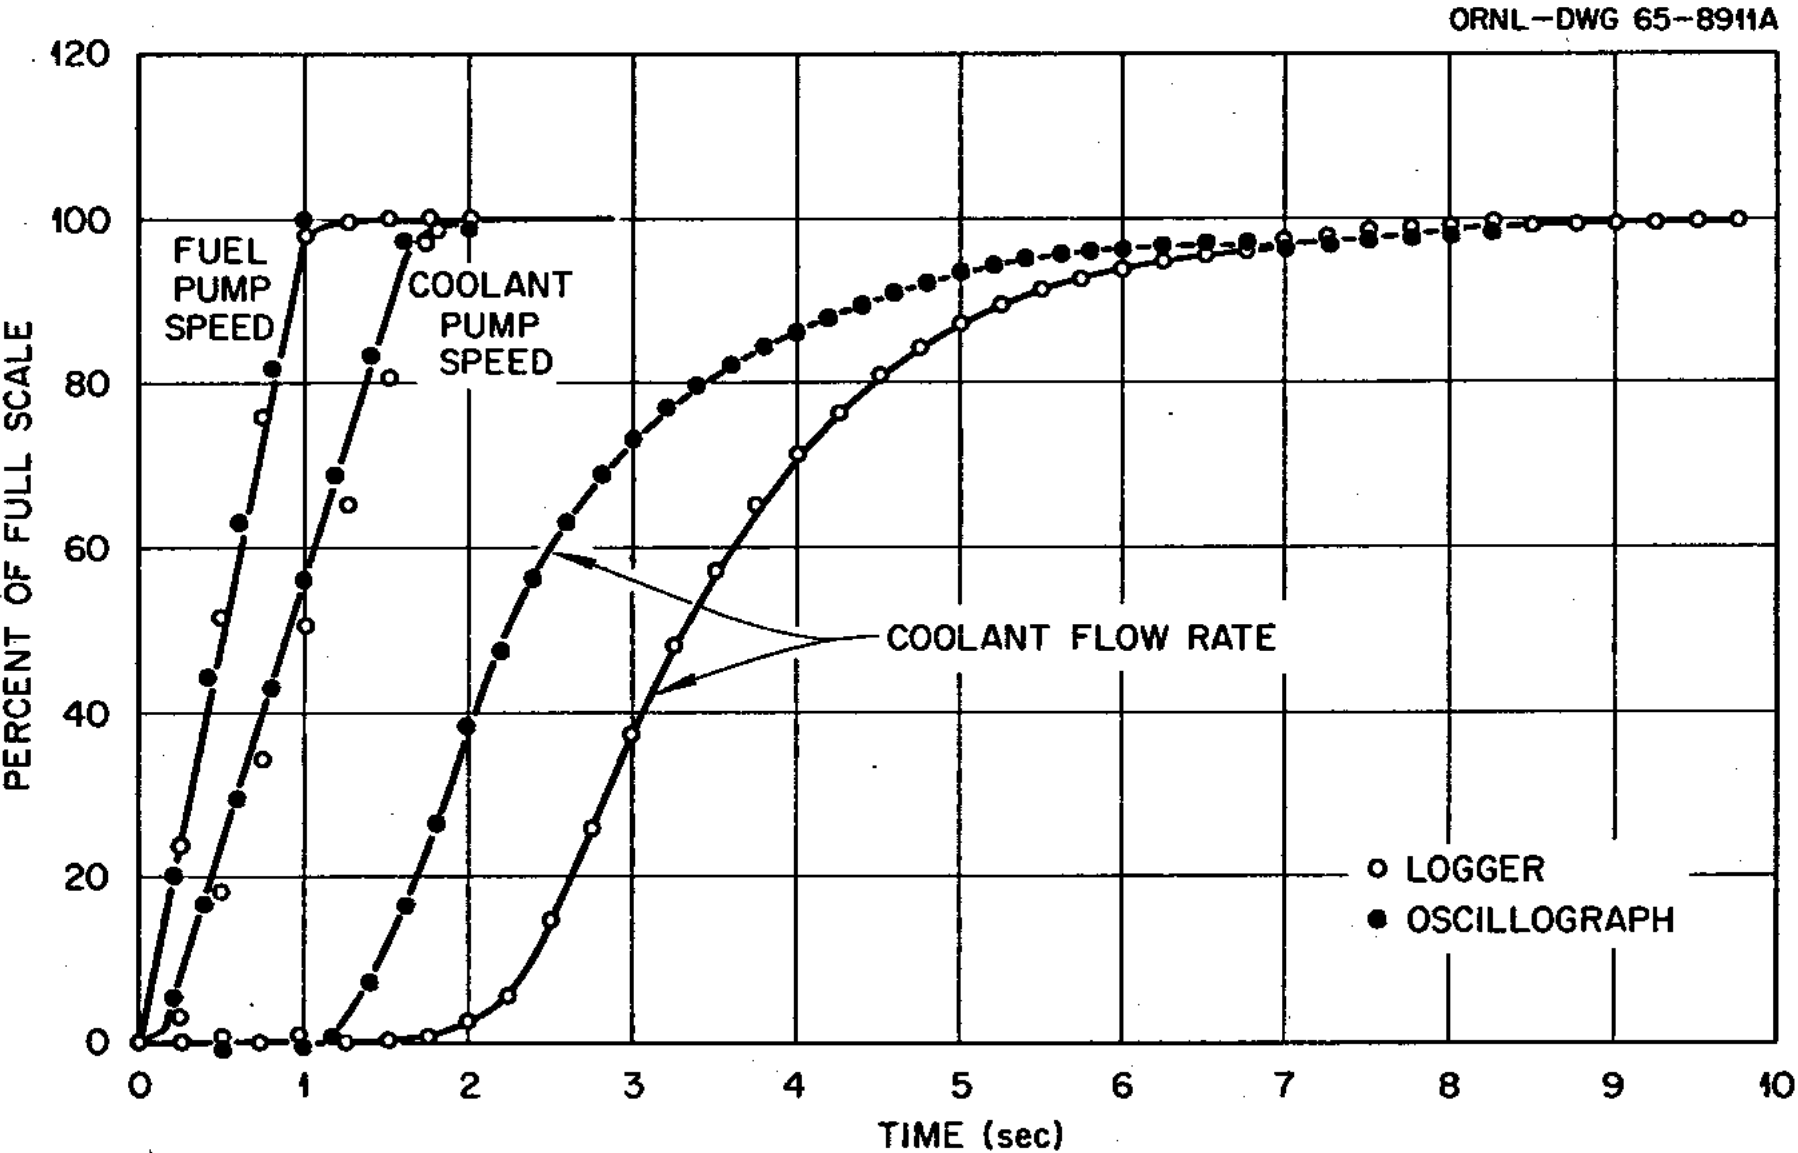
\includegraphics[width=\columnwidth]{msre-startup}
    \caption{Start-up pump speed and coolant flow rate \cite{prince_zero-power_1968}.}
    \label{fig:msre-startup}
  \end{minipage}
  \hfill
  \begin{minipage}[t]{0.49\textwidth}
    \centering
    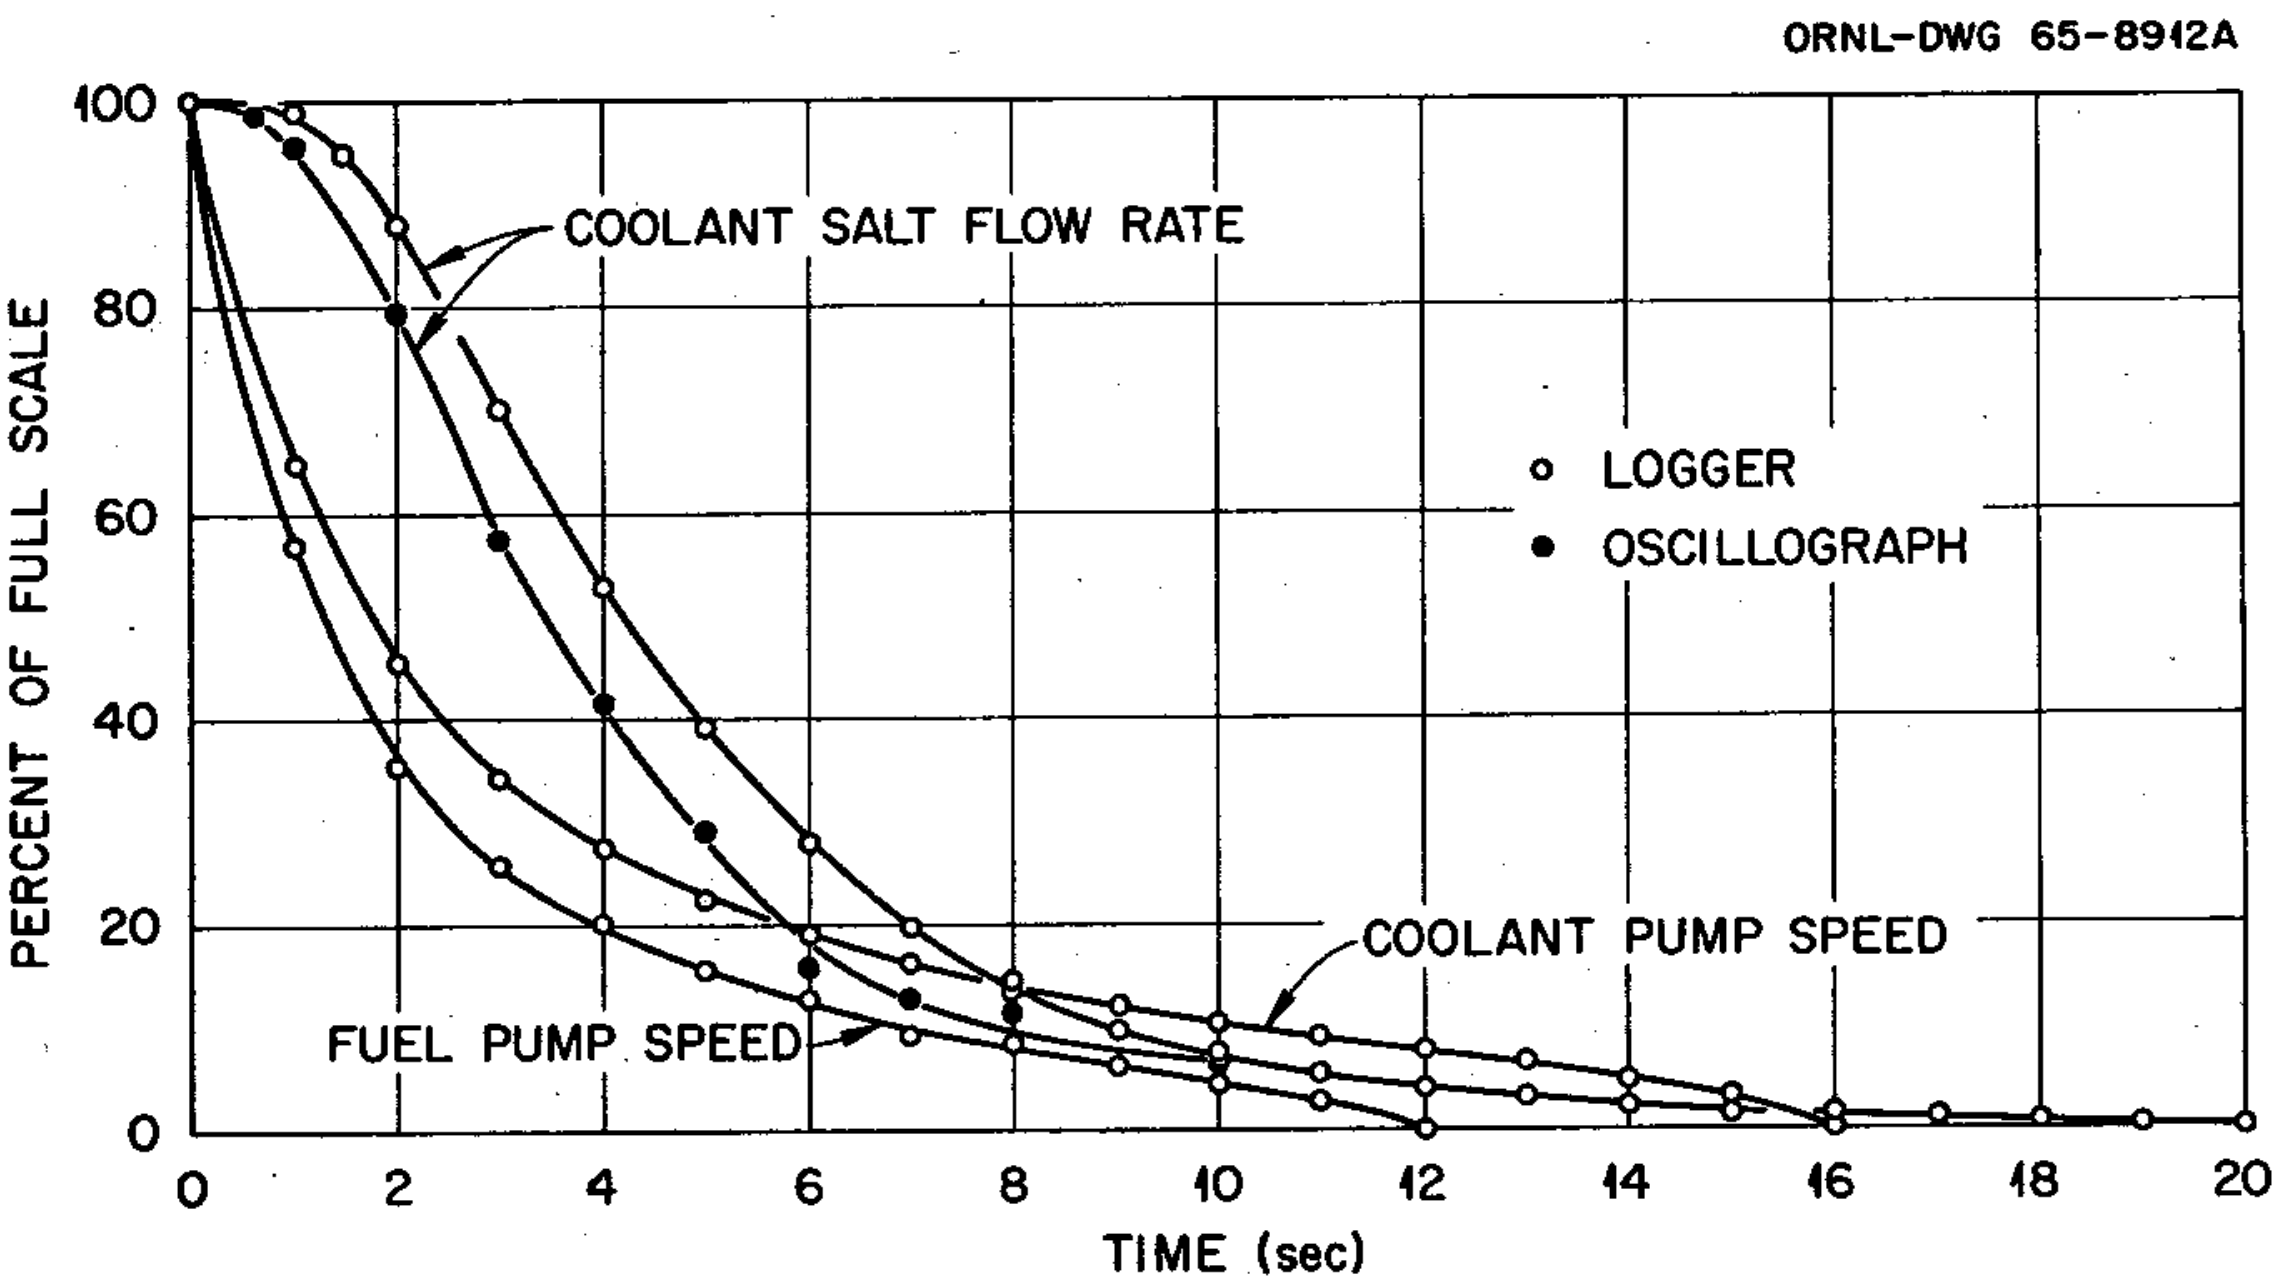
\includegraphics[width=\columnwidth]{msre-coastdown}
    \caption{Coast-down pump speed and coolant flow rate \cite{prince_zero-power_1968}.}
    \label{fig:msre-coastdown}
  \end{minipage}
\end{figure}

\gls{ORNL} researchers performed fuel pump start-up and coast-down transient experiments to
determine the ``transient effects of fuel flow-rate changes on reactivity''
\cite{prince_zero-power_1968}. These experiments were a part of \gls{MSRE} zero-power dynamics
tests performed in June 1965, the same month the \gls{MSRE} achieved initial criticality. Figures
\ref{fig:msre-startup} and \ref{fig:msre-coastdown} show the pump speeds and secondary salt coolant
flow rates measured during the transients. The changing flow rates caused advective changes to the
\gls{DNP} distribution and the \gls{DNF} in the reactor core.

During both experiments, the reactivity effects of the \gls{DNP} drift were measured by
allowing the flux servo controller to maintain criticality. The controller maintained core
criticality by adjusting the control rod insertion height in response to \gls{DNP} drift-induced
reactivity changes. The reactivity changes over time can be calculated by comparing the various
control rod positions (Figure \ref{fig:msre-pump-rod}) with the control rod integral worth curve
(Figure \ref{fig:msre-rod-worth}) obtained during control rod calibration experiments.

\begin{figure}[htb]
  \centering
  \begin{minipage}[t]{0.49\textwidth}
    \centering
    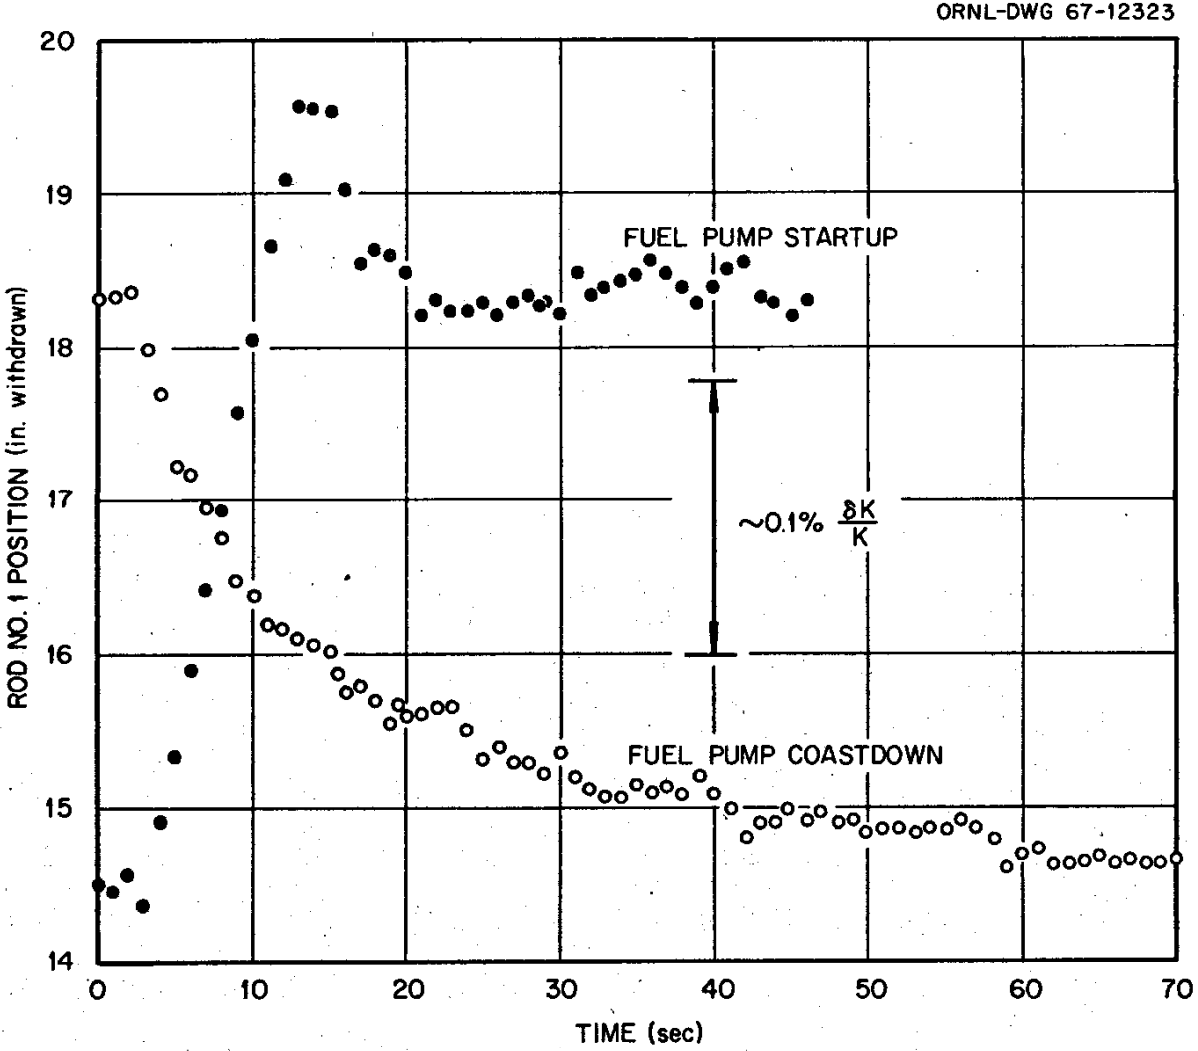
\includegraphics[width=\columnwidth]{msre-transient}
    \caption{Control rod response to fuel pump start-up and coast-down
    \cite{prince_zero-power_1968}.}
    \label{fig:msre-pump-rod}
  \end{minipage}
  \hfill
  \begin{minipage}[t]{0.49\textwidth}
    \centering
    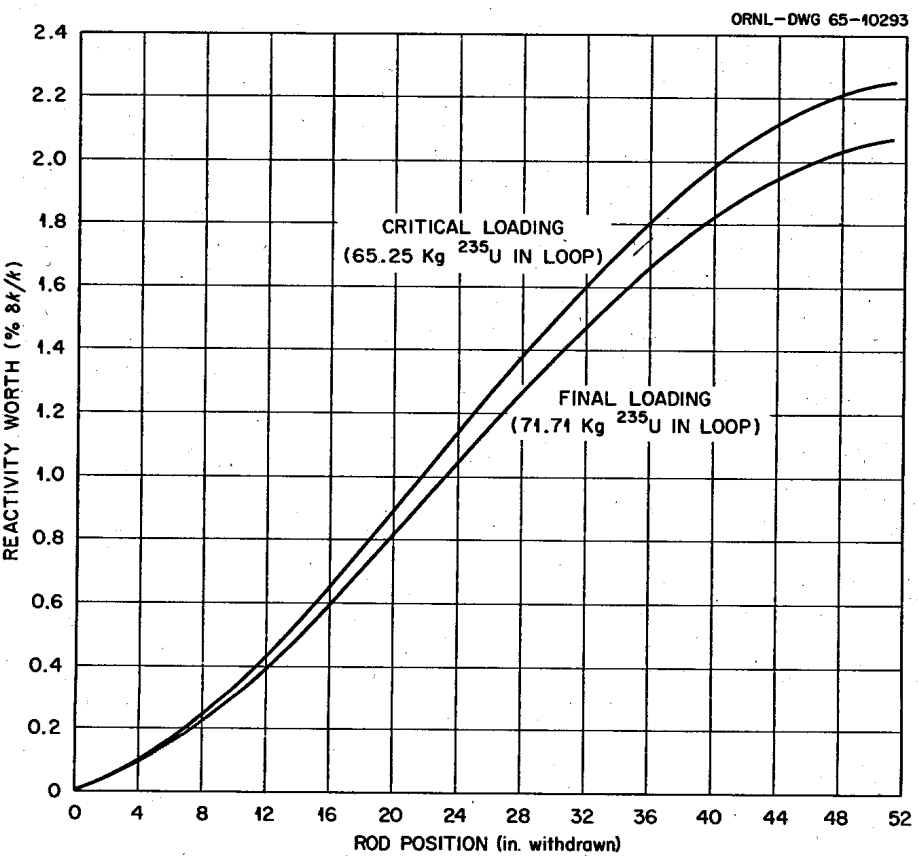
\includegraphics[width=\columnwidth]{msre-rod-worth}
    \caption{Integral control rod worth of Rod 1 \cite{prince_zero-power_1968}.}
    \label{fig:msre-rod-worth}
  \end{minipage}
\end{figure}

\subsection{Description of Reactor Software}

Section \ref{sec:moltres-description} provides general details on the neutronics and \gls{DNP}
models implemented with \gls{FEM} in Moltres. In this study, the neutron flux and \gls{DNP}
variables were approximated using continuous 1st-order Lagrange and discontinuous 2nd-order
monomial basis functions, respectively. The calculations for the neutron flux in the core,
\gls{DNP} in the core, and \gls{DNP} outside the core were tightly coupled using the fixed point
iteration capability available through the MOOSE MultiApp system \cite{gaston_physics-based_2015}.

QuasiMolto \cite{reynolds_analysis_2023} is an open-source multiphysics research code for
simulating circulating fuel reactor kinetics. It uses the multilevel \gls{QD} methodology described
in Section \ref{sec:lit-tc} to model multigroup neutron transport with \gls{DNP} flow and
temperature advection-diffusion. Consisting of three levels of neutron calculations, the highest
level solves the multigroup high-order transport equations for Eddington and boundary factors which
populate previously unknown quantities in the mid-level multigroup low-order \gls{QD} equations.
In turn, the mid-level equations solve for group-collapsed Eddington and boundary factors for the
low-level effective low-order transport equations. The effective low-order transport equations
couple with the \gls{DNP} and temperature governing equations for multiphysics reactivity feedback
from temperature and \gls{DNP} flow. Readers may refer to the linked reference
\cite{reynolds_analysis_2023} for more details on QuasiMolto.

QuasiMolto applies the simple corner balance method \cite{adams_subcell_1997} for spatial
discretization. The simple corner balance method is a subcell, finite-volume method that subdivides
each mesh element into four equal subcells on each mesh corner.
For this study, the QuasiMolto \gls{MSRE} model employed $S_2$ neutron transport to facilitate
fair comparisons with the neutron diffusion method in Moltres. For time-dependent \gls{DNP} flow
modeling, QuasiMolto applies implicit Euler scheme for the reaction
and diffusion terms, and explicit Superbee flux limiter scheme for the advection term.

\subsection{Modeling Approach}

For this study, we adopted a 2-D axisymmetric (R-Z) geometry of the \gls{MSRE} consisting of
alternating vertical regions of molten salt and graphite moderator. This is the same \gls{MSRE}
geometry from Reynolds' PhD thesis \cite{reynolds_multilevel_2020} and
journal publication \cite{reynolds_analysis_2023}. Figure \ref{fig:pump-geom} depicts the 2-D
axisymmetric \gls{MSRE} model. The fuel salt channels are 1.25-cm-wide and spaced at 5 cm intervals
in the graphite matrix. The fuel salt volume fraction of this model is 0.236, differing
slightly to the \gls{MSRE} design specification of 0.225 \cite{robertson_msre_1965}. The geometry
mesh is uniform with a width of $\Delta r=0.078125$ cm and height of $\Delta z=5$ cm.
Vacuum boundary conditions for the neutron flux apply along the top, bottom, and right boundaries.

The salt flows
upwards at a spatially uniform velocity rate of 18.085 cm s$^{-1}$. \glspl{DNP} flow out of the
core model and through a separate 285-cm-long 1-D pipe model before being reintroduced through the
bottom core channel inlets. The 1-D pipe length maintains the overall salt circulation time of
25.2 s from the \gls{MSRE} design specification \cite{robertson_msre_1965}. Note that the salt
velocity and 1-D pipe length in this study differs from the \gls{MSRE} model described in Reynolds'
paper \cite{reynolds_analysis_2023}. We reduced the velocity to compensate for the absence of upper
and lower core plena by extending salt residence time in the salt-graphite lattice region.

\begin{figure}[htb]
  \centering
  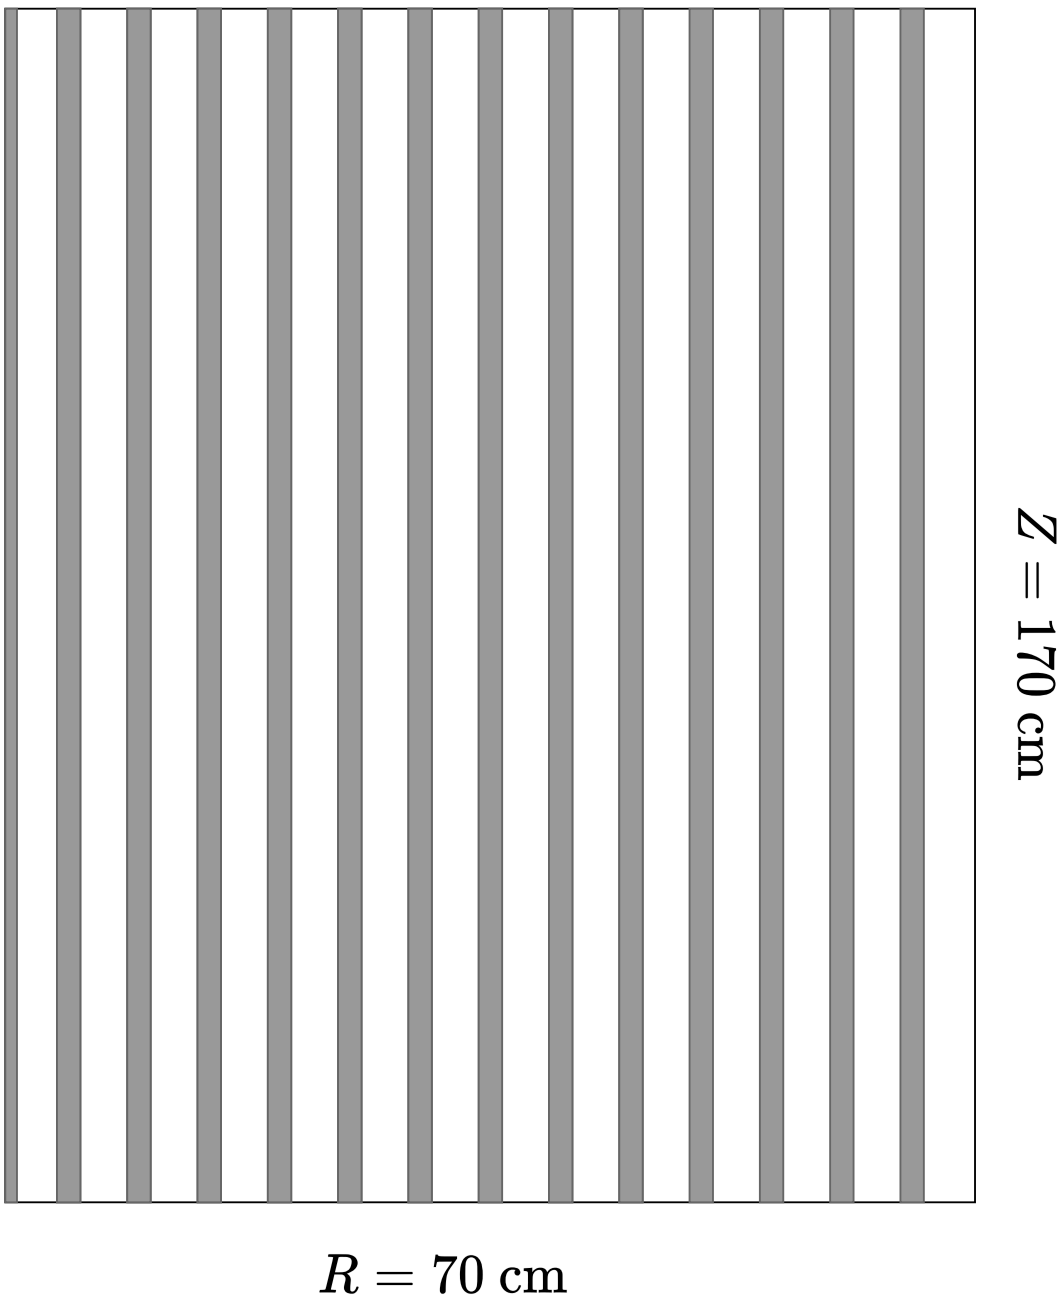
\includegraphics[width=0.6\columnwidth]{msre-2d}
  \caption{2-D axisymmetric model of the \gls{MSRE}.The gray and white regions represent fuel salt
  and graphite, respectively. The leftmost fuel salt channel falls along the axis of symmetry and
  is half-width. Not drawn to scale.}
  \label{fig:pump-geom}
\end{figure}

Reynolds generated group constants for two neutron energy groups and six \gls{DNP} groups using the
NEWT transport module within the SCALE code system \cite{rearden_scale_2018} and the ENDF/B-VII
nuclear data library \cite{chadwick_endf/b-vii.1_2011}. The SCALE model geometry comprised a
representative unit cell geometry
consisting of a circular fuel region in the center of a square graphite region and reflective
boundary conditions on all boundaries. The unit cell dimensions preserved material compositions
and salt-to-graphite ratios from the \gls{MSRE} design specifications.

Prior to the pump transient simulations, we performed code-to-code verification by comparing the
$k_\text{eff}$ and neutron flux and \gls{DNP} distributions of the 2-D \gls{MSRE} model under
static, no salt flow conditions. We sampled the neutron flux and \gls{DNP} distributions on
mesh corners and edge centers along the centerline ($r=0$ cm) and on mesh edge centers along
the midplane ($z=85$ cm) of the reactor geometry.

In lieu of reactivity control using a control rod in the pump
transient simulations, Moltres and QuasiMolto solved their respective
two-group $k$-eigenvalue neutronics models at every time-step. The $1/k_\text{eff}$ scaling factor
in the fission neutron source term keeps the simulation at a pseudo-critical state. The \gls{DNP}
source term is also scaled by $1/k_\text{eff}$ at every time-step. We interpolated the \gls{MSRE}
salt flow velocity data in Figures \ref{fig:msre-startup} and \ref{fig:msre-coastdown} to apply in
our pump start-up and coast-down simulations. The pump start-up simulation starts from a static
state with no salt flow while the pump coast-down simulation starts from a steady flow state with
operating salt flow. Both simulations used a fixed time-step size of 0.1 s.

\subsection{Results \& Discussion}

We start with a comparison of the Moltres and QuasiMolto \gls{MSRE} numerical models under static
and steady salt flow conditions. Table \ref{table:msre-pump-keff} lists the $k_\text{eff}$
estimates under static and steady flow conditions, and the reactivity changes due to \gls{DNP}
flow. Moltres and QuasiMolto show excellent agreement with 22 and 21 pcm absolute differences in
$k_\text{eff}$ under static and steady flow conditions, respectively. Consequently, the
$\Delta\rho$ estimates from \gls{DNP} flow fall within less than 1 pcm difference of each other.

\begin{table}[htb]
  \centering
  \caption{Multiplication factors $k_\text{eff}$ under static and steady salt flow conditions, and
  reactivity changes $\Delta\rho$ due to \gls{DNP} flow from the Moltres and QuasiMolto \gls{MSRE}
  models.}
  \begin{tabular}{l S S S}
    \toprule
    \multirow{2}{*}{Code} & \multicolumn{2}{c}{$k_\text{eff}$} & {$\Delta\rho$ due to} \\
                          & {Static} & {Steady flow} & {\gls{DNP} flow} \\
                          \cmidrule(r){1-1} \cmidrule(rl){2-3} \cmidrule(l){4-4}
    Moltres & 1.05625 & 1.05311 & -282.4 \\
    QuasiMolto & 1.05603 & 1.05290 & -281.7 \\
    \bottomrule
  \end{tabular}
  \label{table:msre-pump-keff}
\end{table}

Moving on to comparing spatial distributions, we start with the centerline neutron flux
distributions. Figure \ref{fig:centerline-flux-dist} shows the normalized group 1 and 2 neutron
fluxes exhibiting nearly perfect overlap. The QuasiMolto-to-Moltres flux ratio distributions in
Figure \ref{fig:centerline-flux-ratio} illustrate the strong agreement between Moltres and
QuasiMolto at all sampled locations with the relative differences falling below 0.8\%. We attribute
the oscillations in the flux ratios to differences in spatial discretization schemes. Moltres
uses \gls{FEM} with 1st-order flux values computed at the mesh corners. QuasiMolto uses
the simple corner balance method which subdivides each mesh element into four equal subcells and
computes volume-averaged flux values in each subcell. As such, Moltres and QuasiMolto require
interpolation for sampling mesh edge center and mesh corner values, respectively. The flux ratios
sampled at the top and bottom boundaries show the greatest differences of up to 0.8\%. We attribute
these differences at the boundaries to differences in neutronics methods. The neutron diffusion
method vacuum boundary condition in Moltres depends on the scalar flux gradient (1-st
order derivative) while the $S_2$ method vacuum boundary condition in QuasiMolto depends on the
angular flux value. Combined with the different spatial discretization schemes, flux differences at
the boundary are expected in numerical calculations. Nevertheless, the overall ratio magnitudes
remain small, thereby showing that Moltres and QuasiMolto are consistent with each other.

\begin{figure}[t]
  \centering
  \begin{subfigure}[b]{0.48\columnwidth}
    \centering
    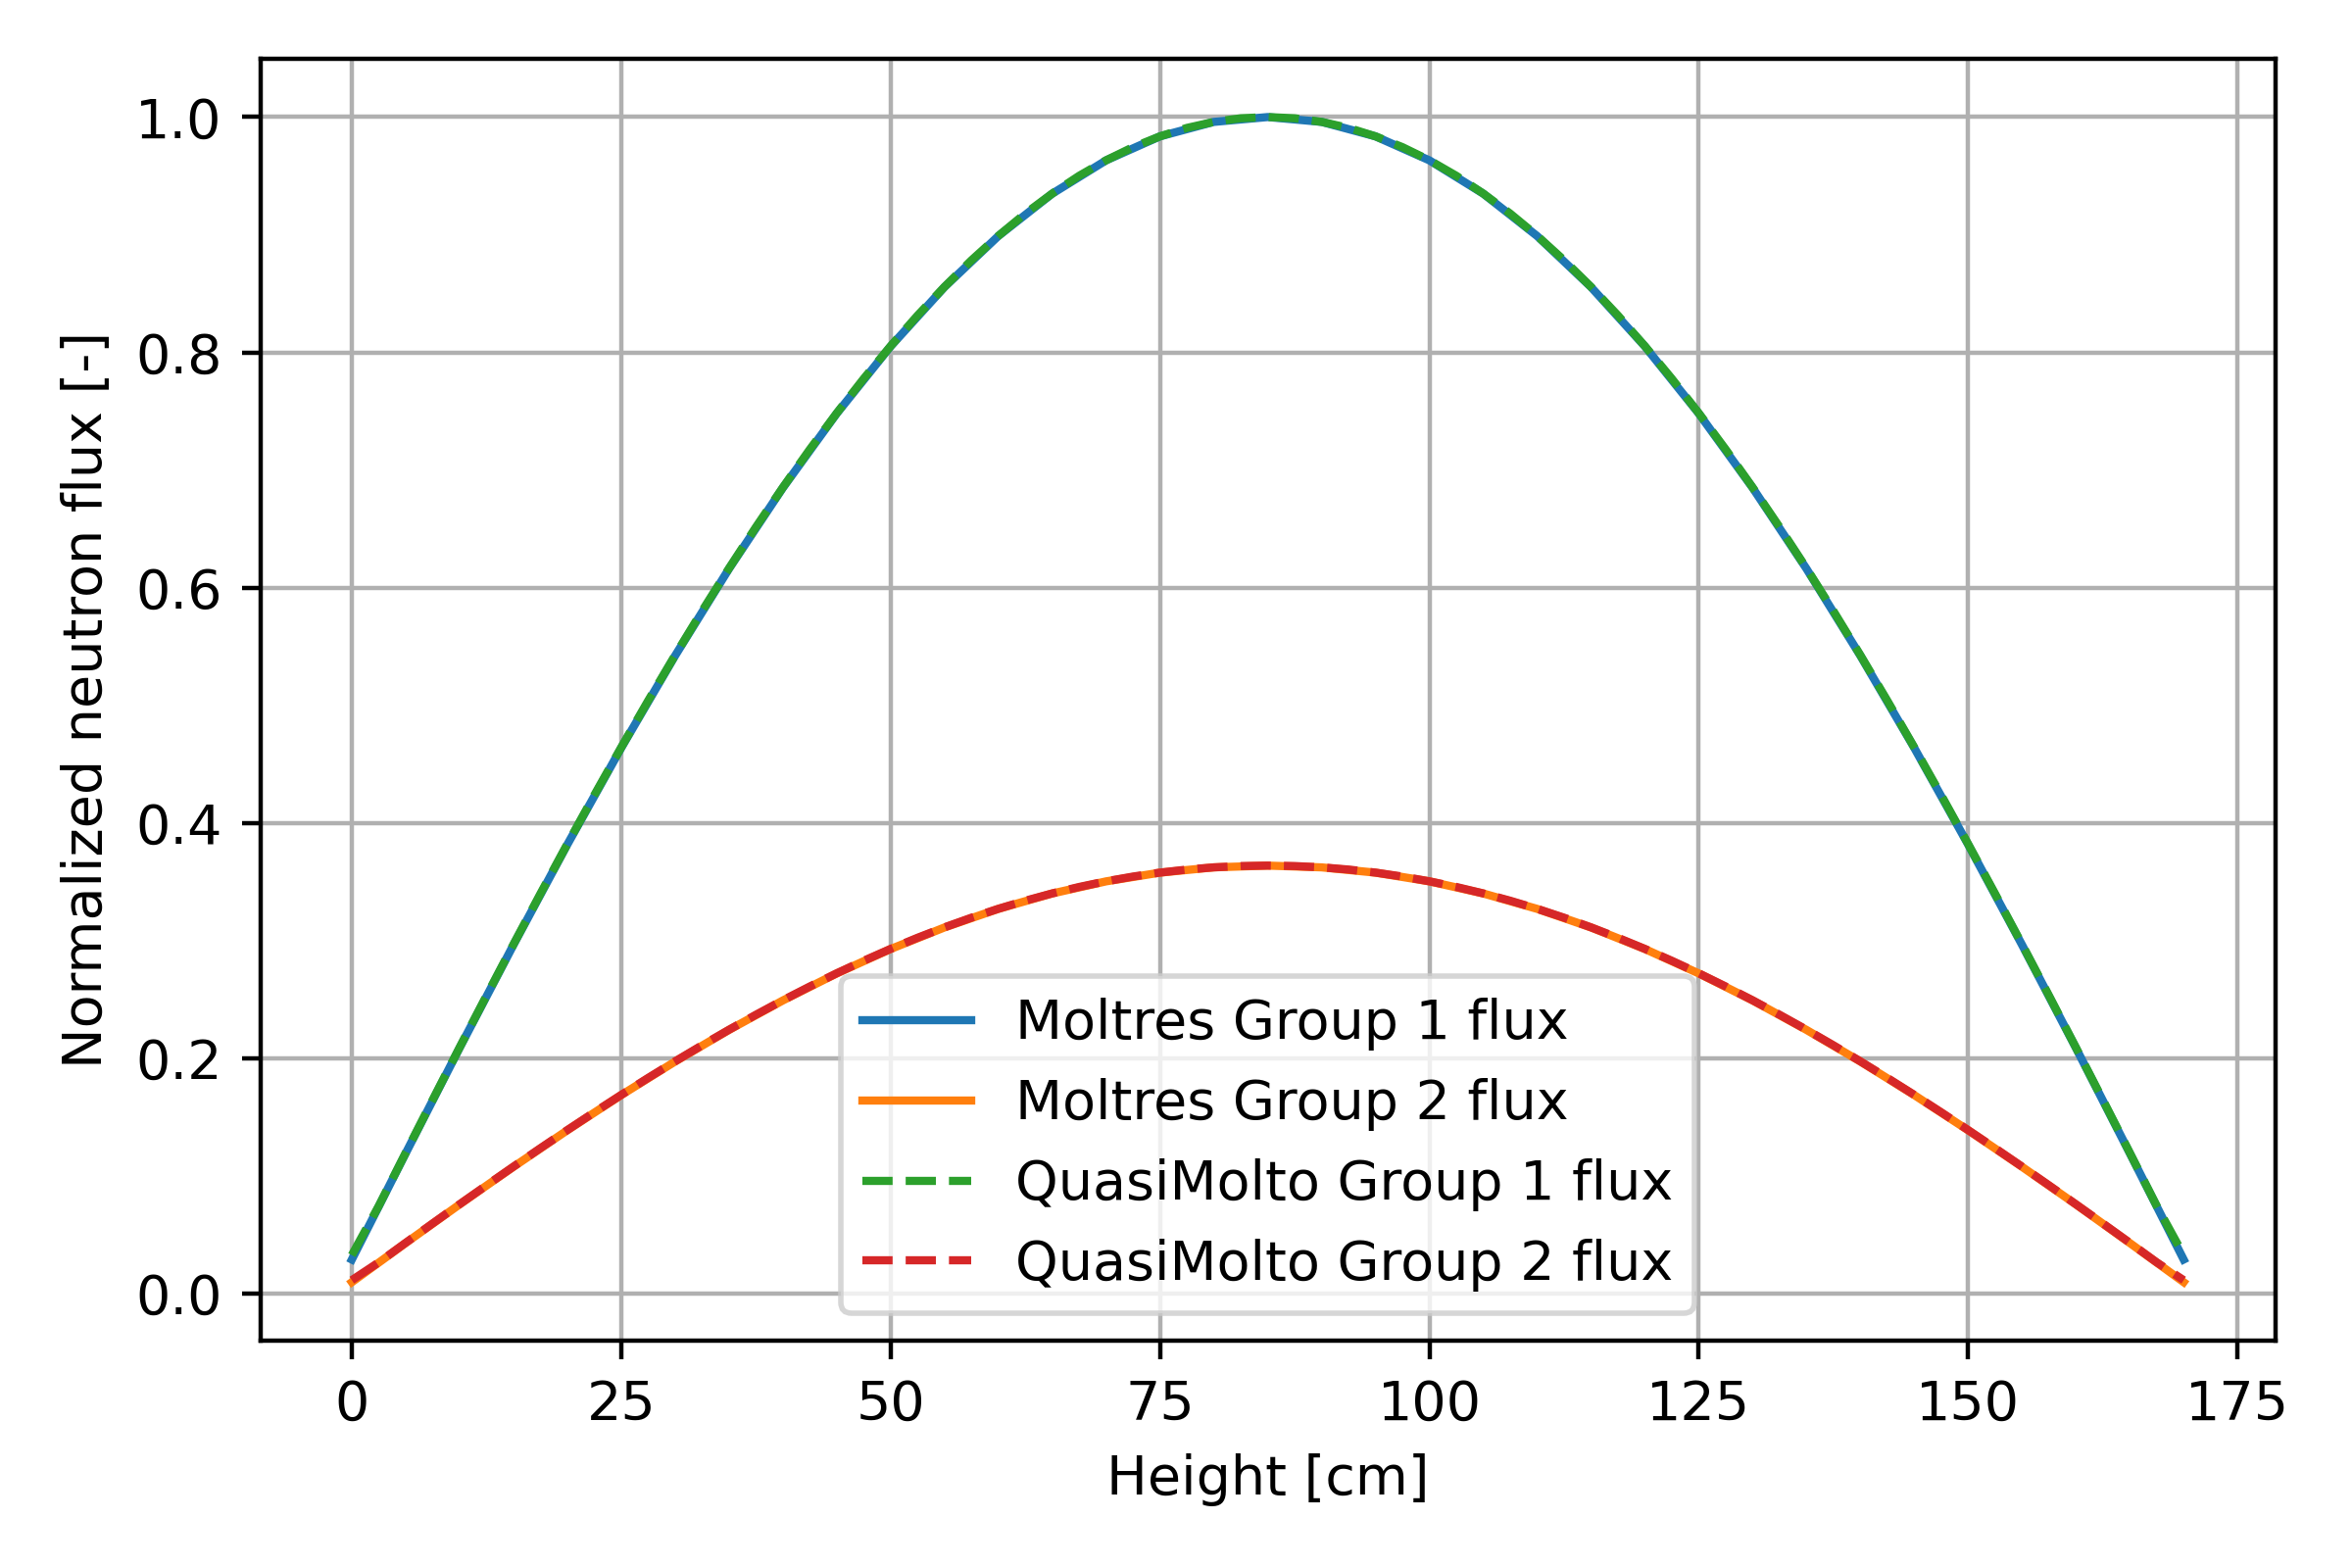
\includegraphics[width=\columnwidth]{centerline_flux}
    \caption{Normalized centerline neutron fluxes.}
    \label{fig:centerline-flux-dist}
  \end{subfigure}
  \hfill
  \begin{subfigure}[b]{0.48\columnwidth}
    \centering
    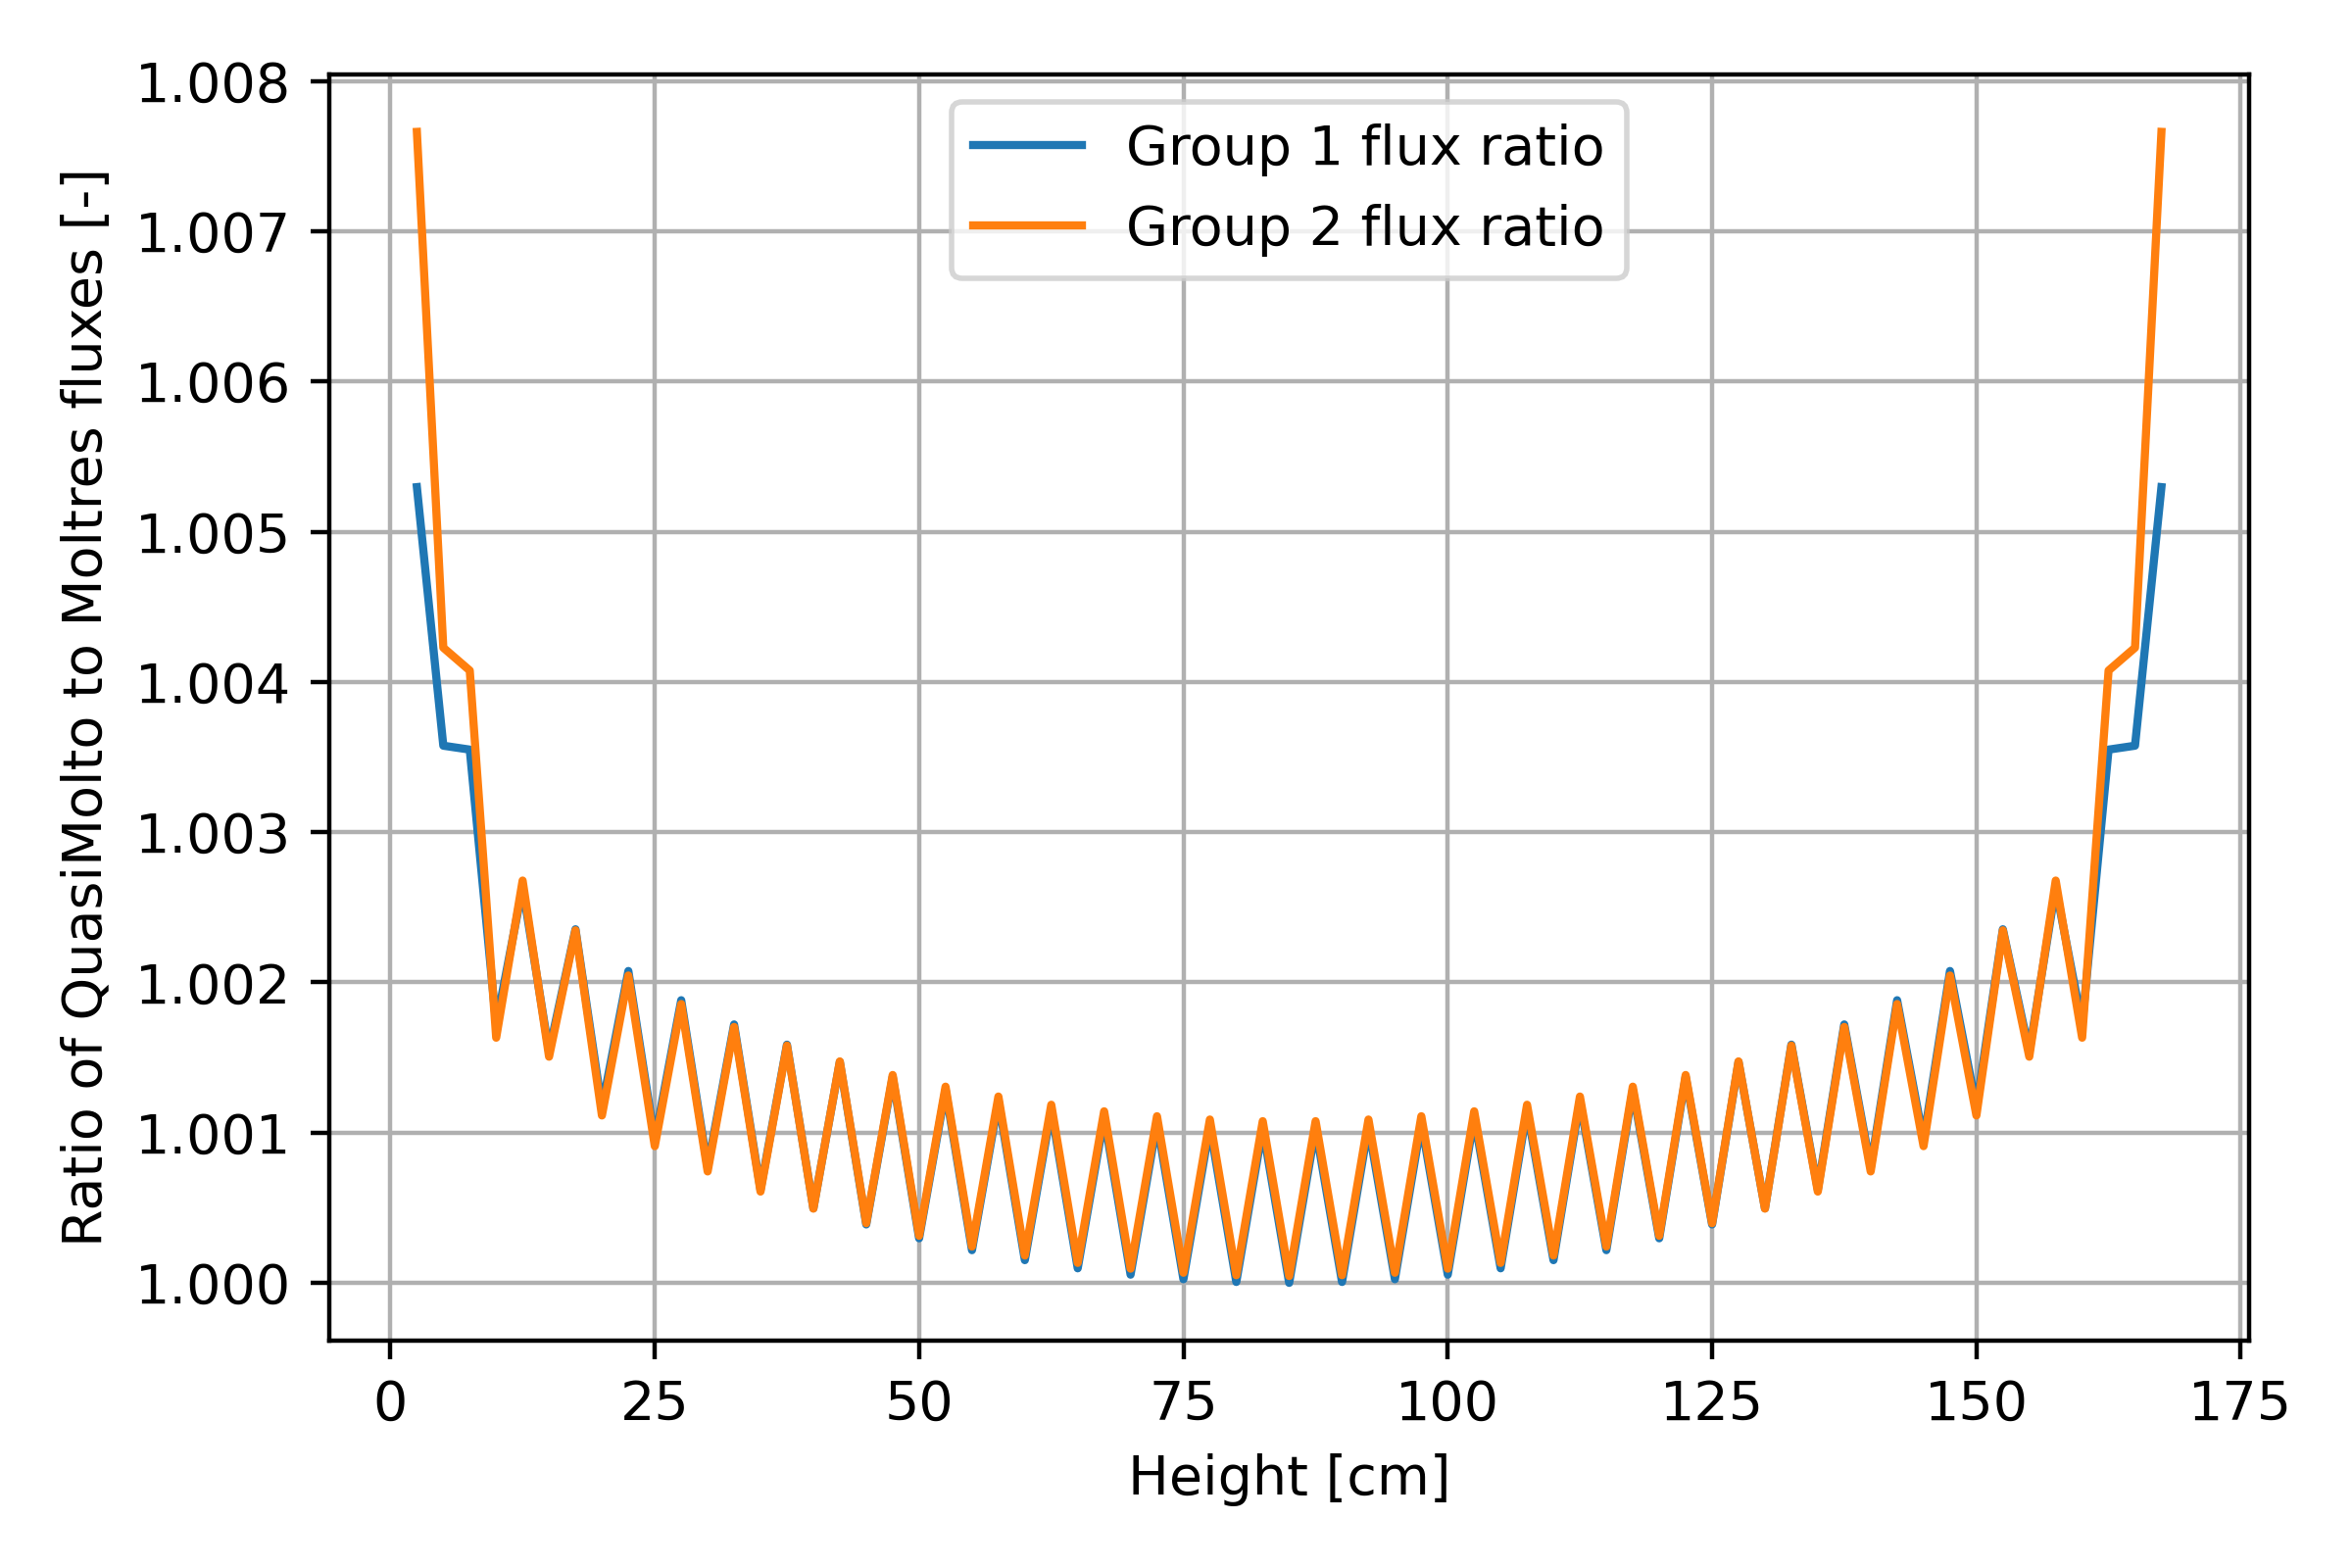
\includegraphics[width=\columnwidth]{centerline_flux_ratio}
    \caption{Ratio of centerline neutron fluxes.}
    \label{fig:centerline-flux-ratio}
  \end{subfigure}
  \caption{Centerline neutron flux distributions and ratios comparing QuasiMolto and Moltres
  \gls{MSRE} models under static conditions.}
  \label{fig:centerline-flux}
  \begin{subfigure}[b]{0.48\columnwidth}
    \centering
    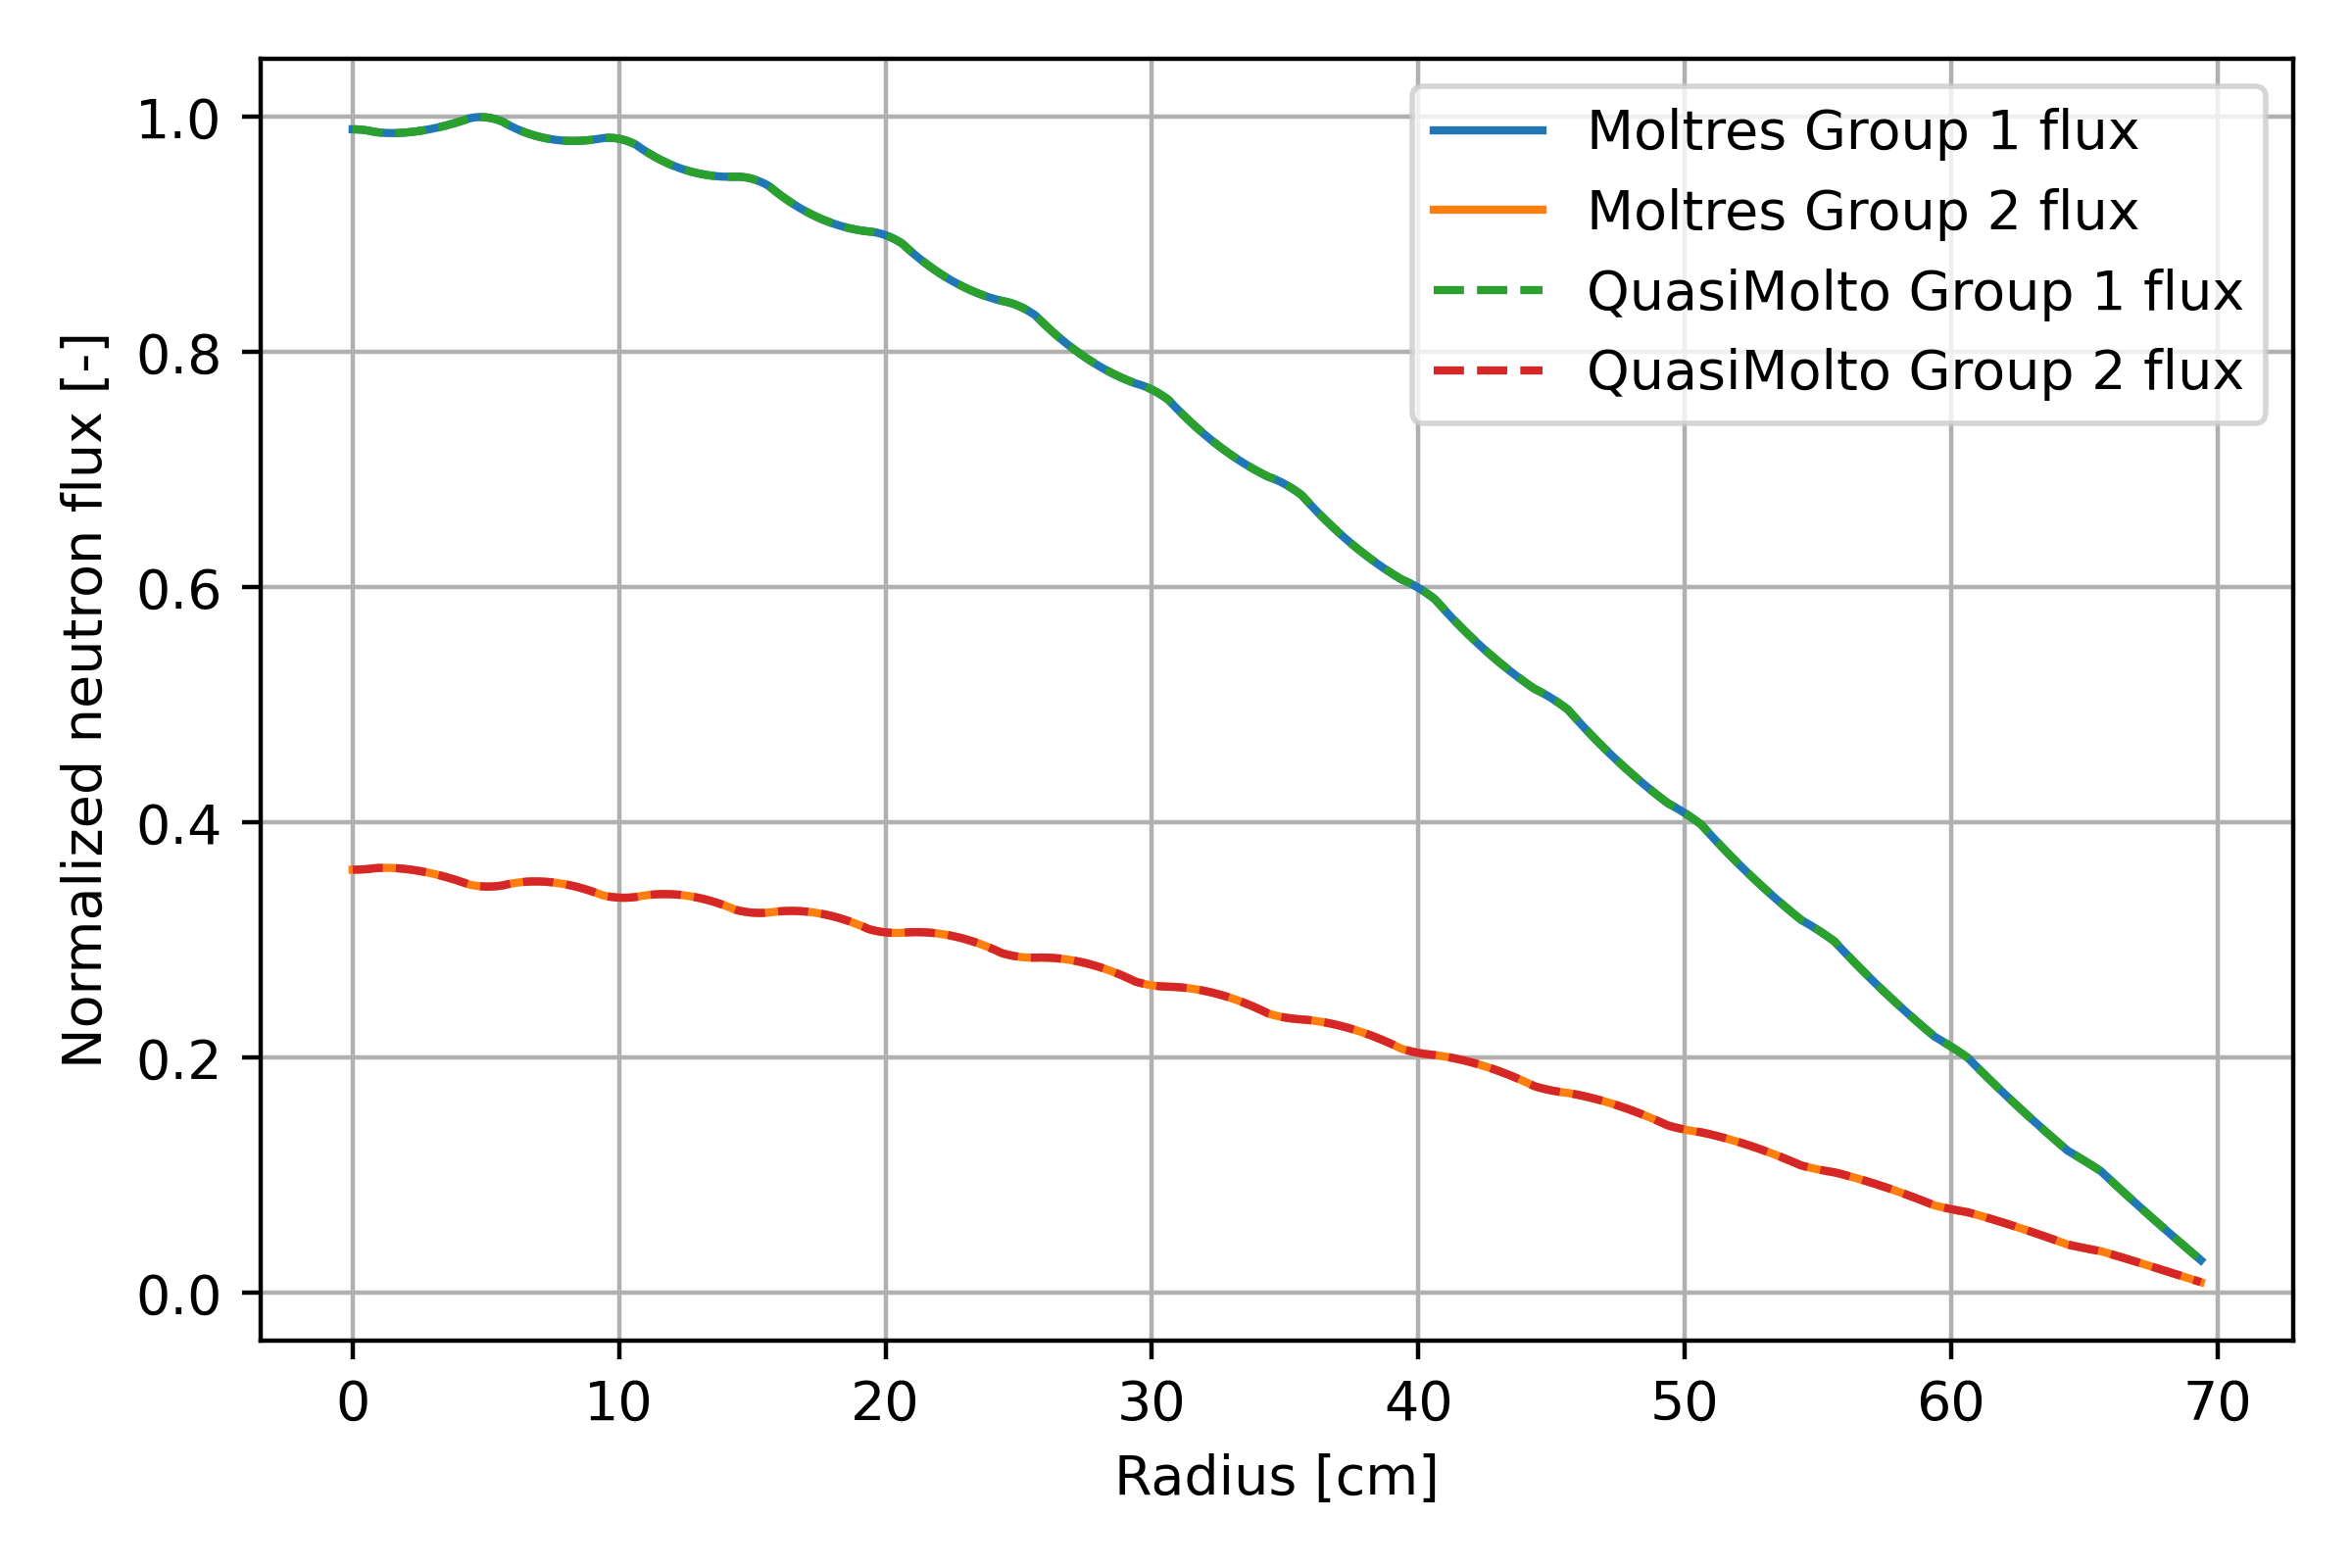
\includegraphics[width=\columnwidth]{midplane_flux}
    \caption{Normalized midplane neutron fluxes.}
    \label{fig:midplane-flux-dist}
  \end{subfigure}
  \hfill
  \begin{subfigure}[b]{0.48\columnwidth}
    \centering
    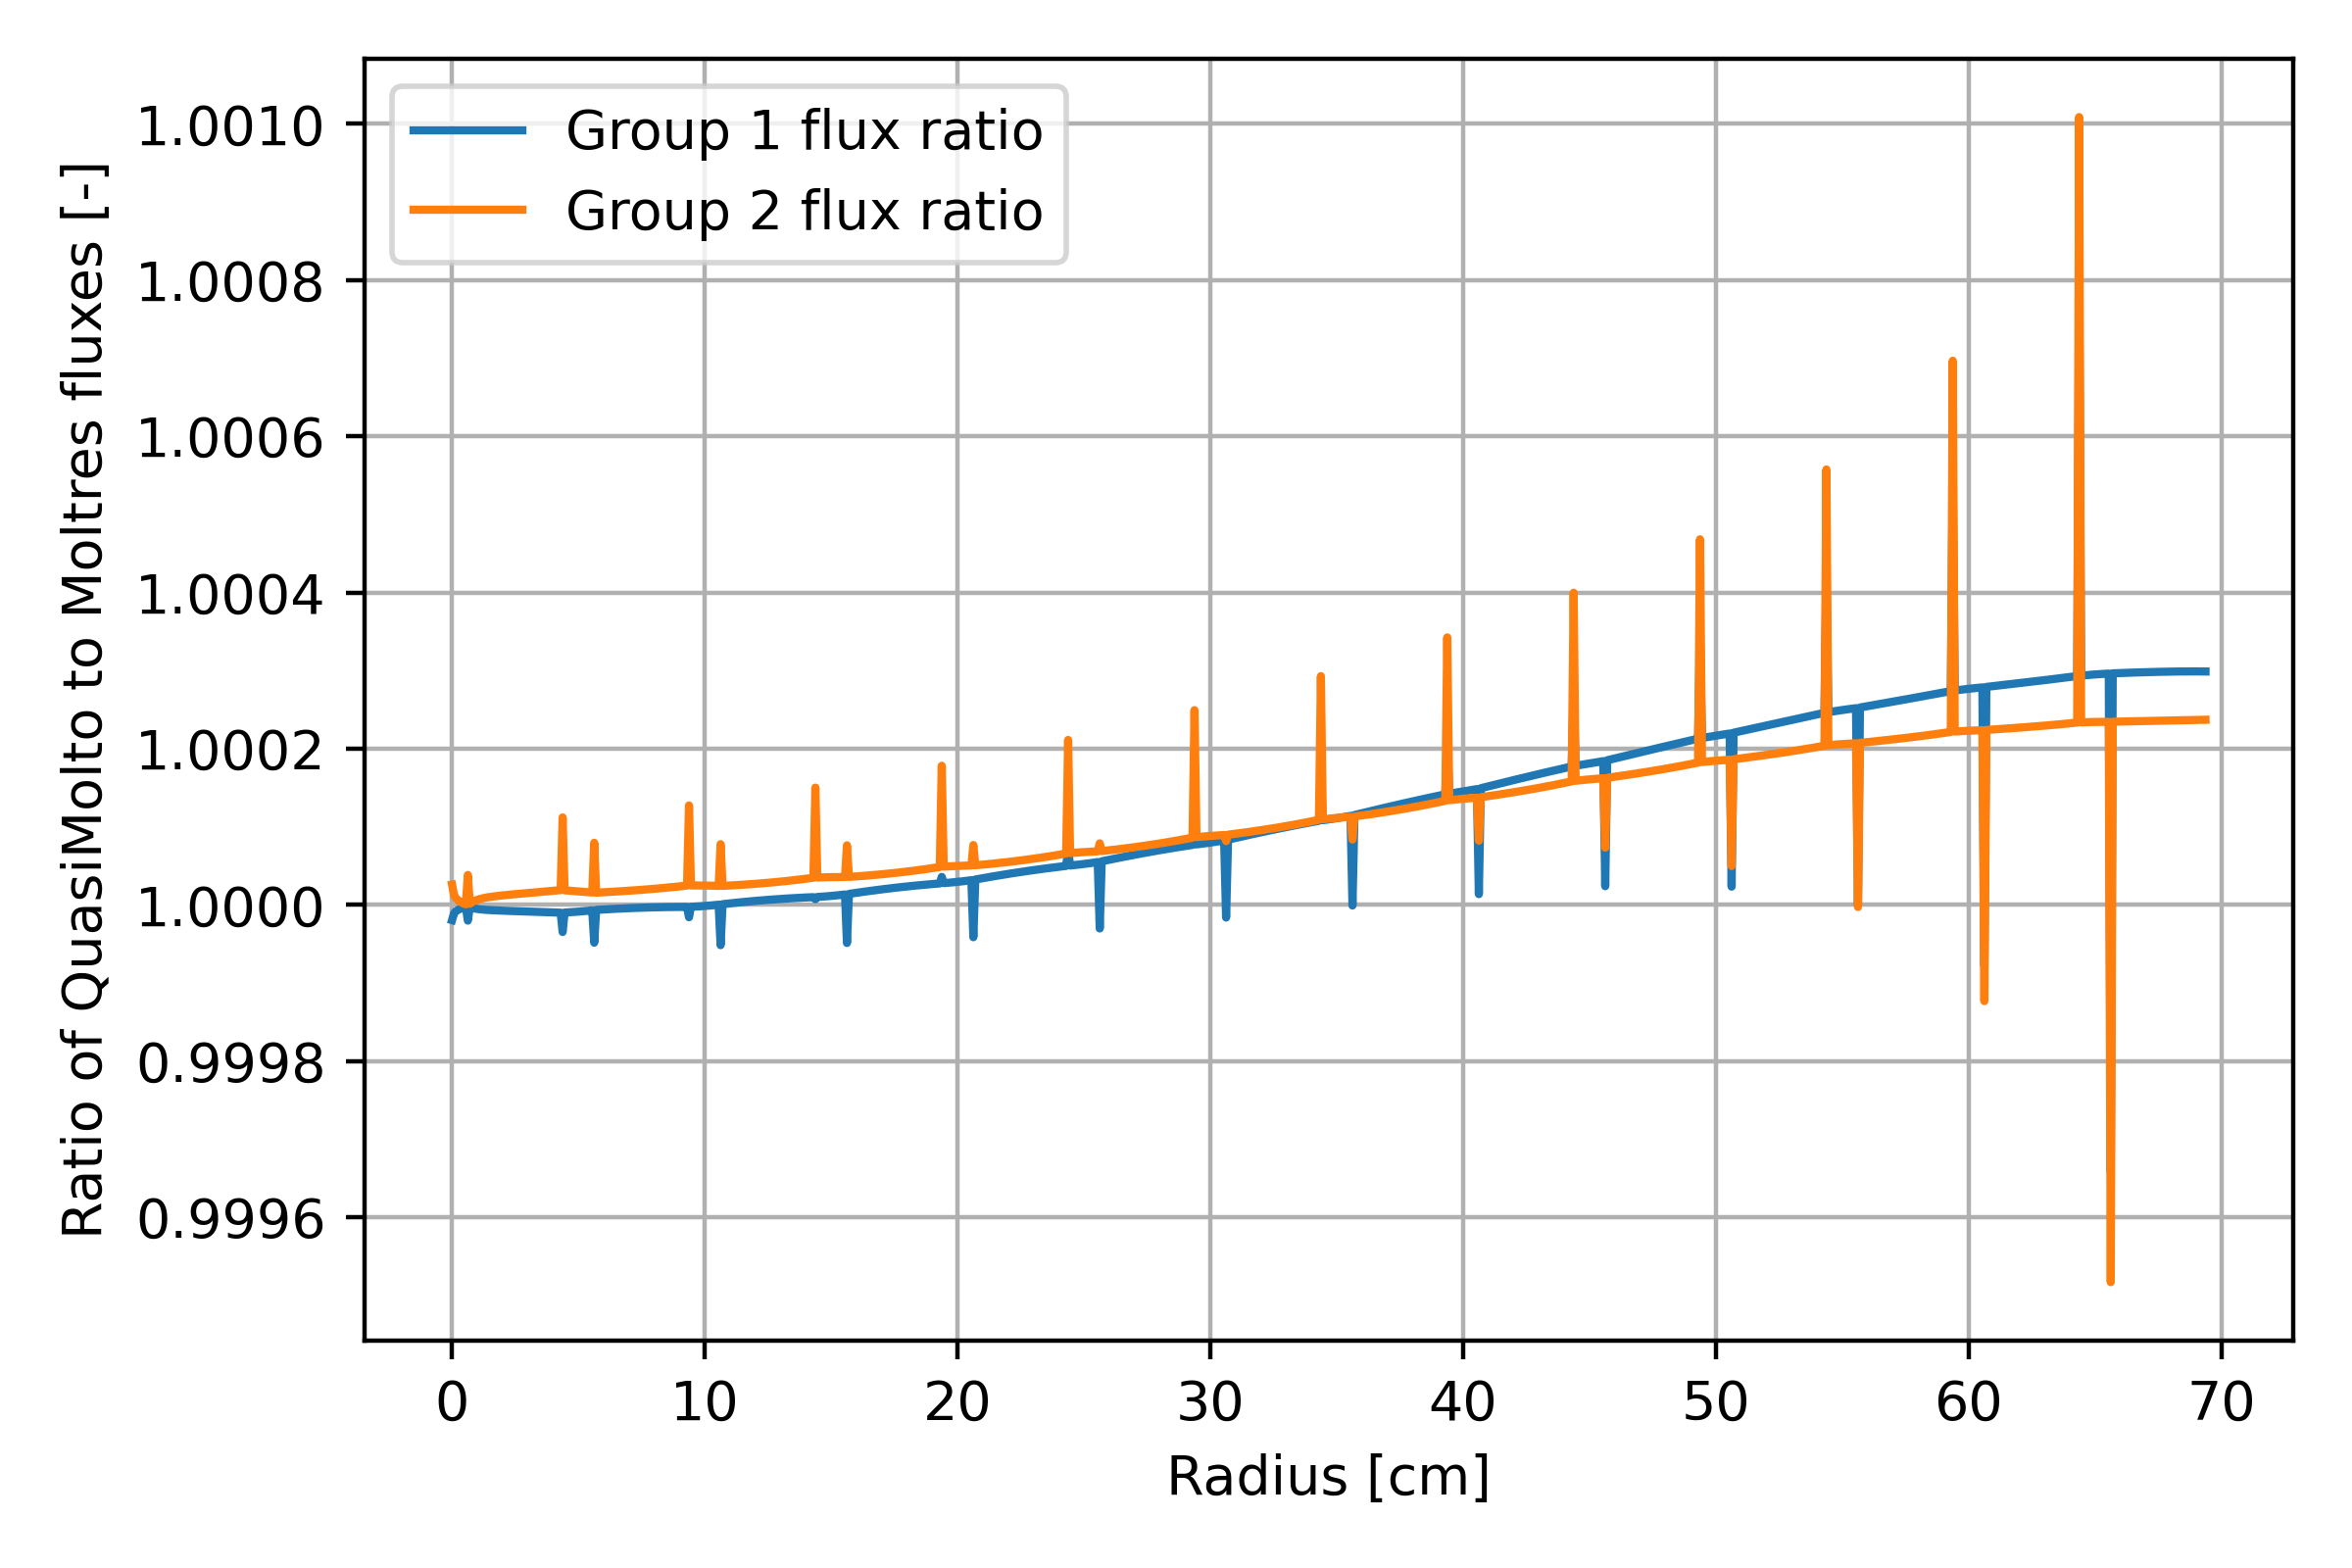
\includegraphics[width=\columnwidth]{midplane_flux_ratio}
    \caption{Ratio of midplane neutron fluxes.}
    \label{fig:midplane-flux-ratio}
  \end{subfigure}
  \caption{Midplane neutron flux distributions and ratios comparing QuasiMolto and Moltres
  \gls{MSRE} models under static conditions.}
  \label{fig:midplane-flux}
\end{figure}

The midplane normalized neutron flux and flux ratio distributions in Figures
\ref{fig:midplane-flux-dist} and \ref{fig:midplane-flux-ratio} also show consistency between
Moltres and QuasiMolto through nearly perfect flux overlap and small flux ratios. Minor
discretization errors arising from comparing continuous (Moltres) and discontinuous (QuasiMolto)
fluxes contribute to discrete jumps in the flux ratios at the salt-graphite interfaces. Despite
these deviations,
the maximum midplane flux ratio of 1.001 remains much lower than the maximum centerline flux ratio
of 1.008. Fine mesh resolution along the radial direction helps the vacuum boundary flux values
converge. The centerline and midplane \gls{DNP} distributions and ratios in Figures
\ref{fig:centerline-pre} and \ref{fig:midplane-pre} continue to show good agreement between Moltres
and QuasiMolto. Figures \ref{fig:centerline-pre-dist} and \ref{fig:midplane-pre-dist} depict only
the normalized centerline and midplane \gls{DNP} distributions from Moltres to reduce visual
clutter. Combining all observations thus far, Moltres and QuasiMolto are consistent with each other
under static and steady salt flow conditions.

\begin{figure}[t]
  \centering
  \begin{subfigure}[b]{0.48\columnwidth}
    \centering
    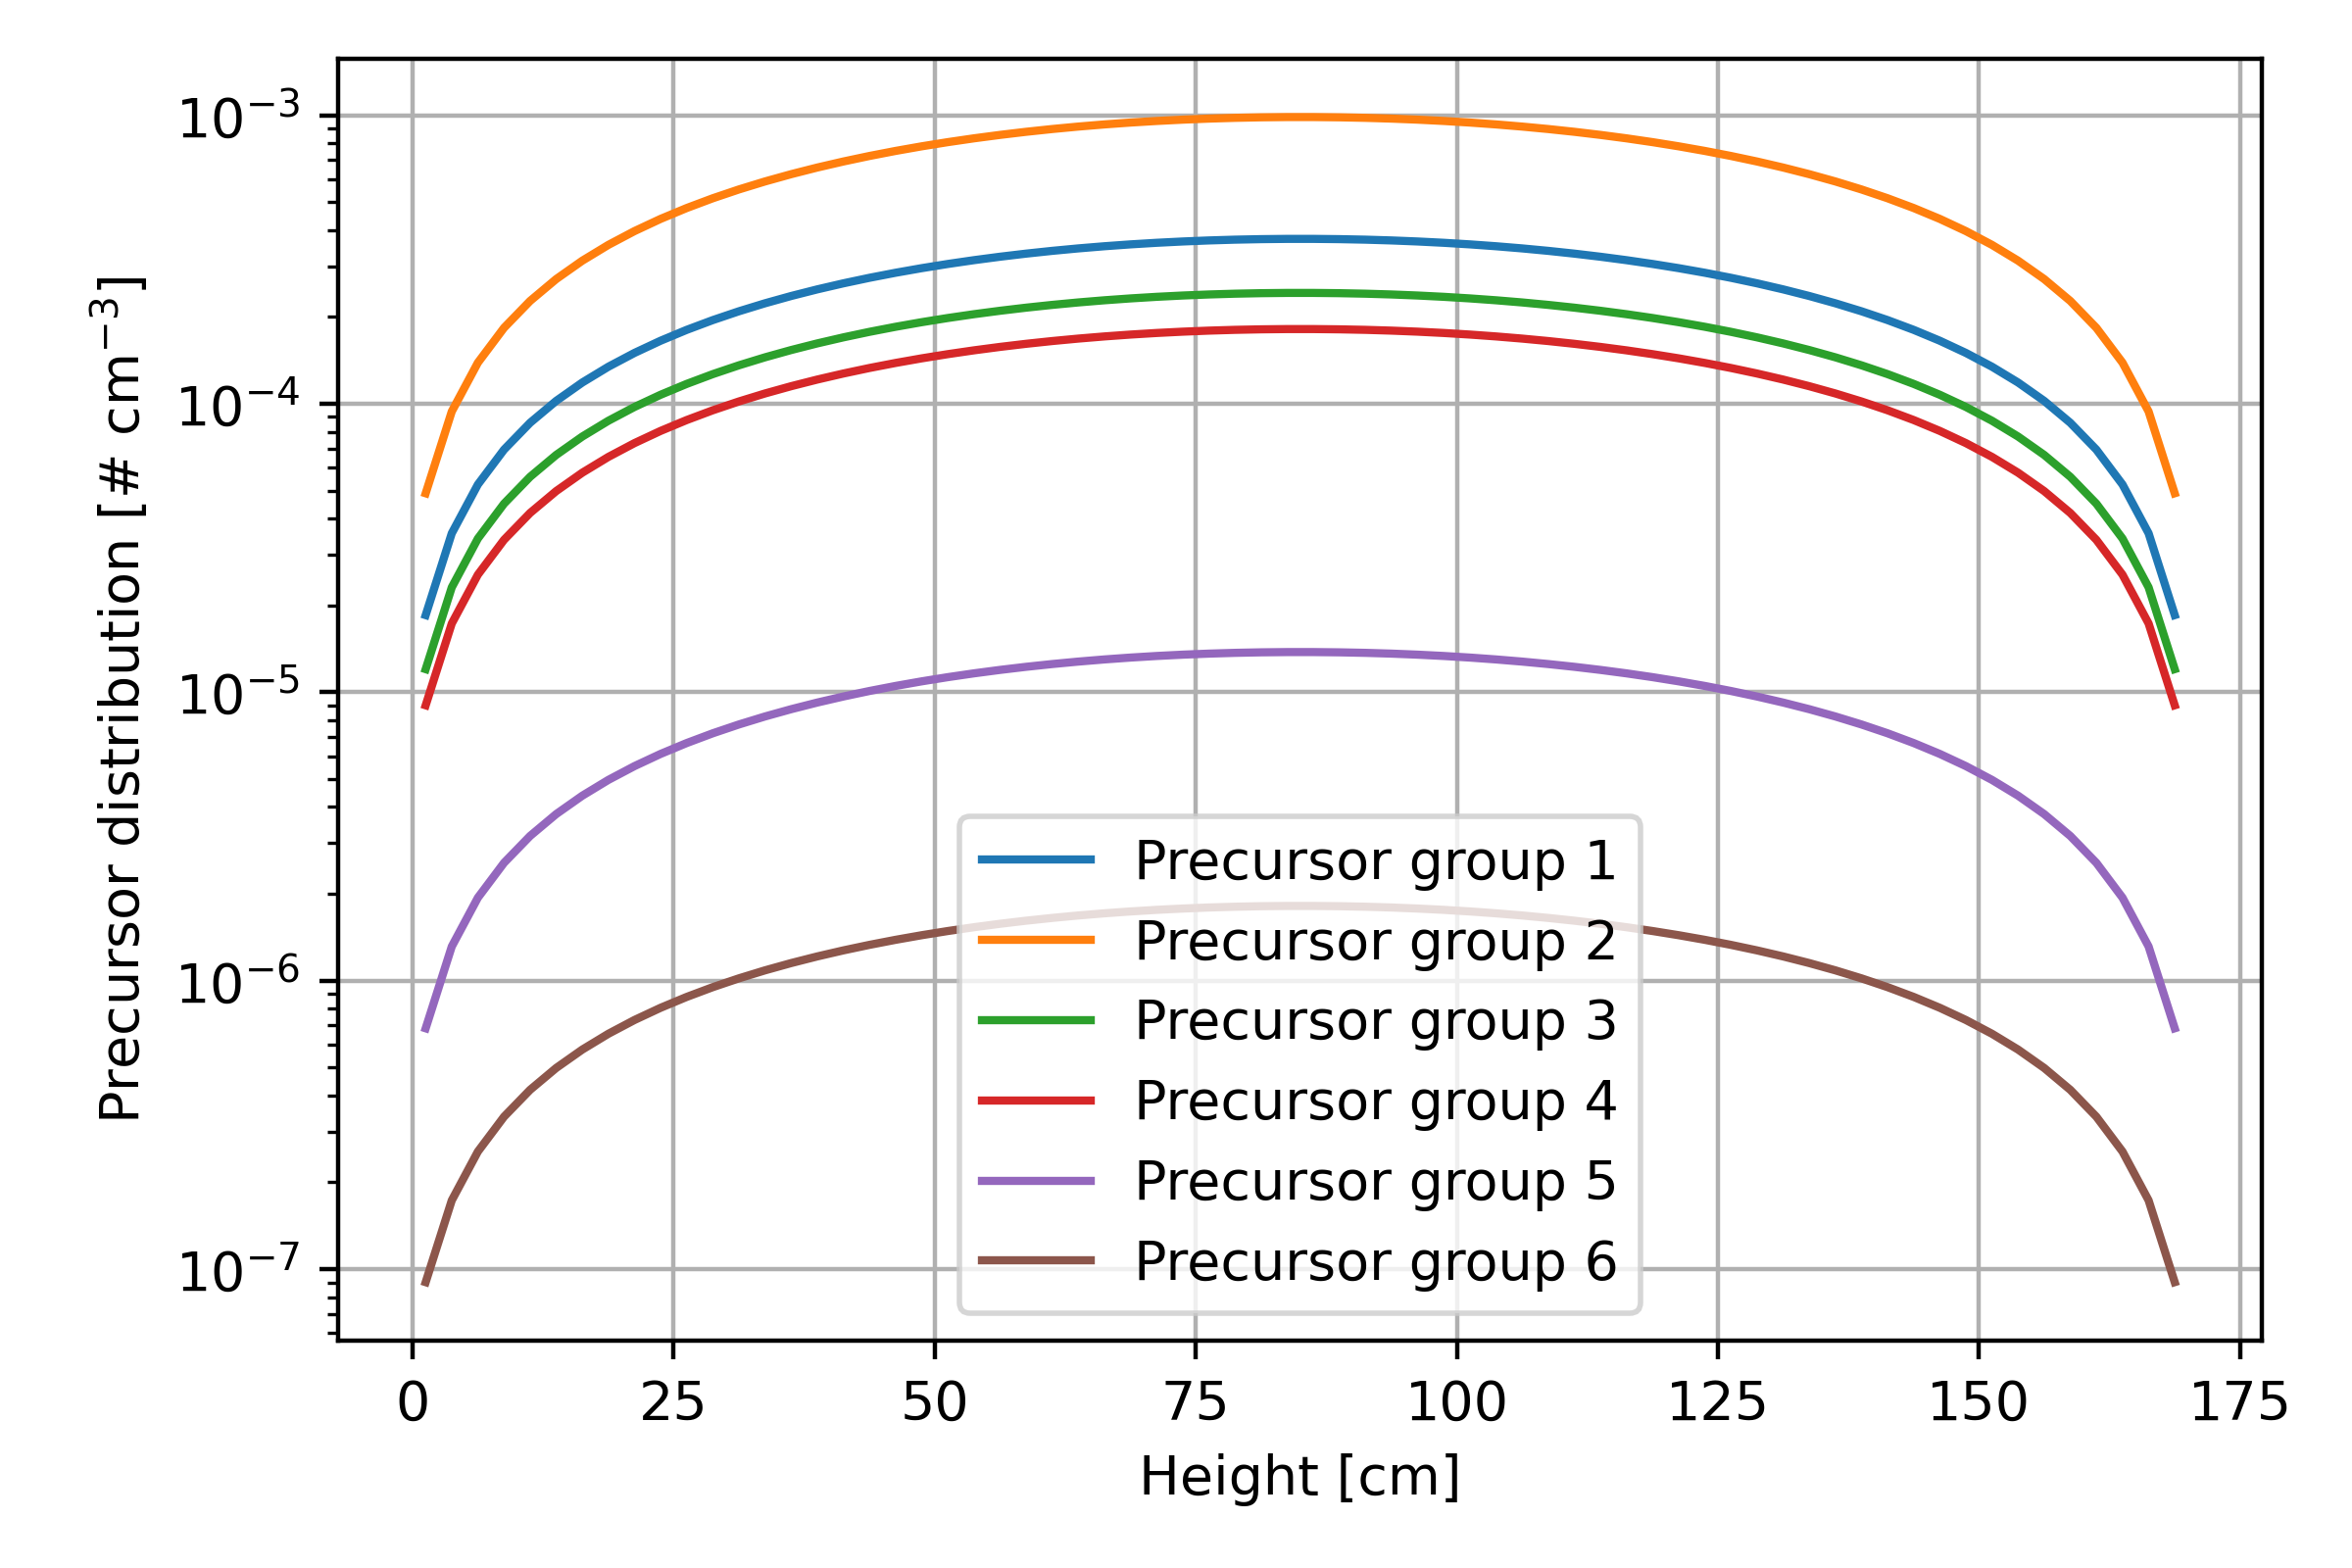
\includegraphics[width=\columnwidth]{centerline_pre}
    \caption{Normalized centerline \gls{DNP} distributions.}
    \label{fig:centerline-pre-dist}
  \end{subfigure}
  \hfill
  \begin{subfigure}[b]{0.48\columnwidth}
    \centering
    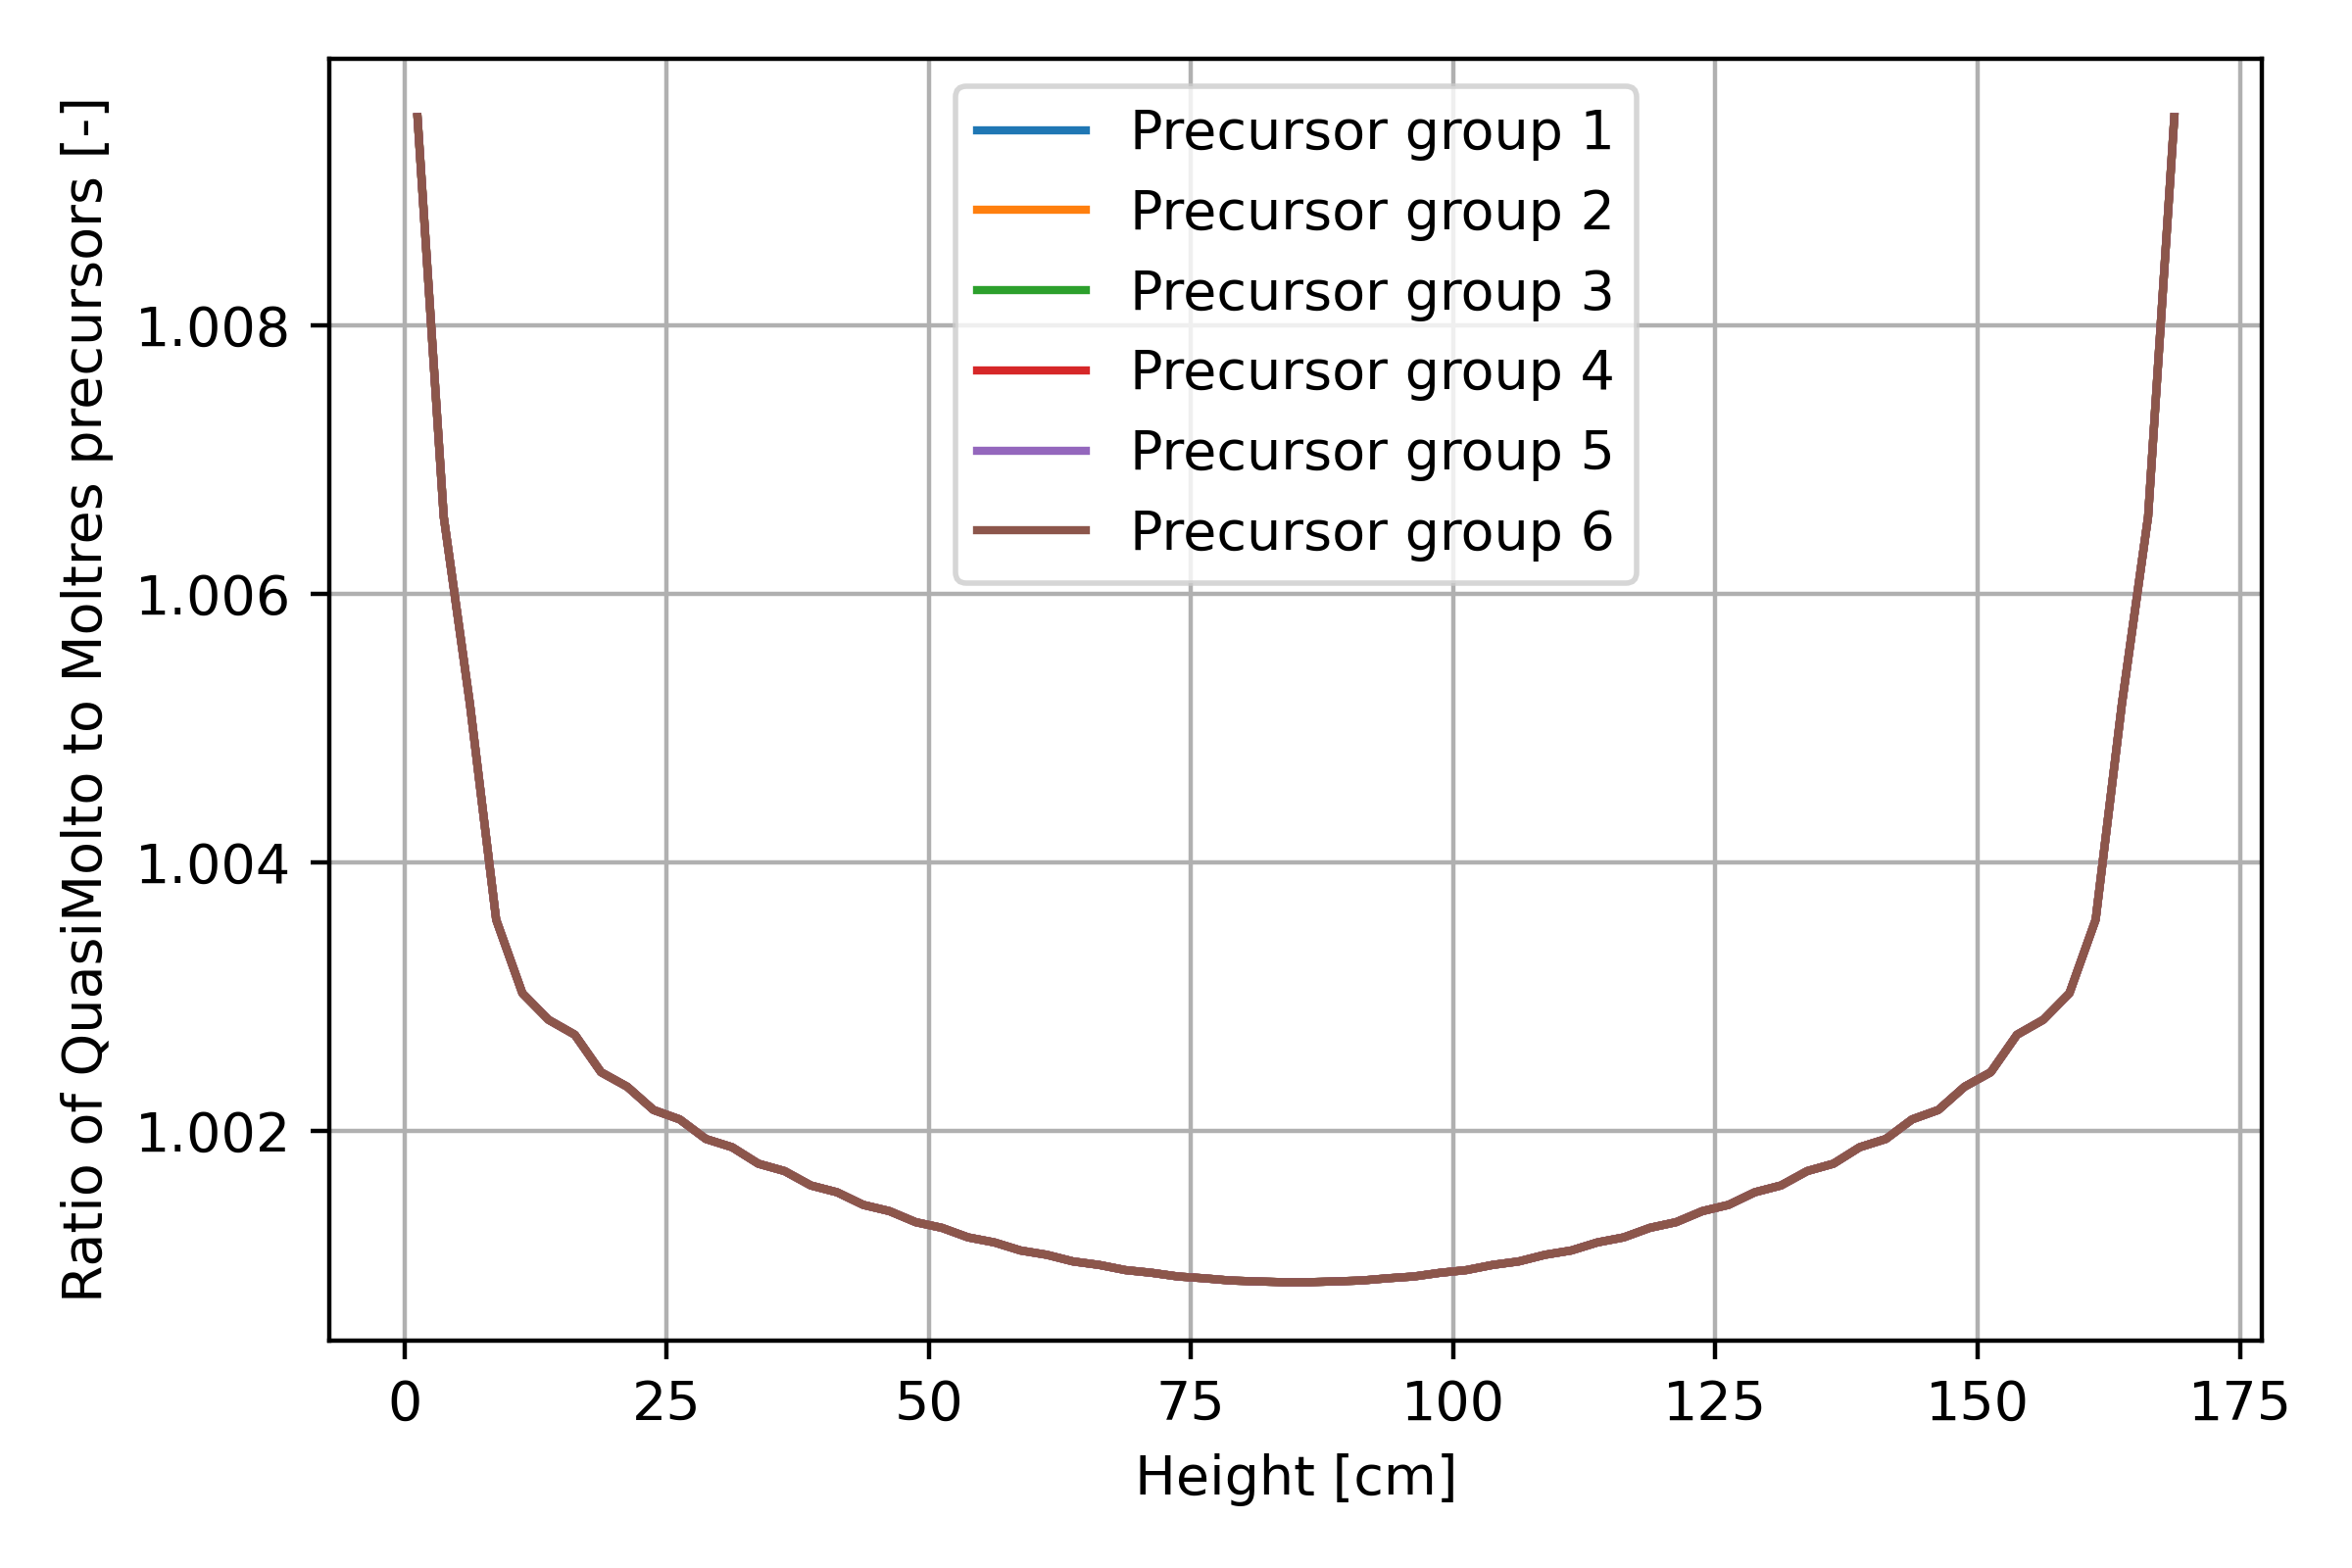
\includegraphics[width=\columnwidth]{centerline_pre_ratio}
    \caption{Ratio of centerline \gls{DNP} distributions.}
    \label{fig:centerline-pre-ratio}
  \end{subfigure}
  \caption{Centerline \gls{DNP} distribution from Moltres and ratios comparing QuasiMolto and
  Moltres models under static \gls{MSRE} conditions. The ratio curves overlap perfectly.}
  \label{fig:centerline-pre}
  \begin{subfigure}[b]{0.48\columnwidth}
    \centering
    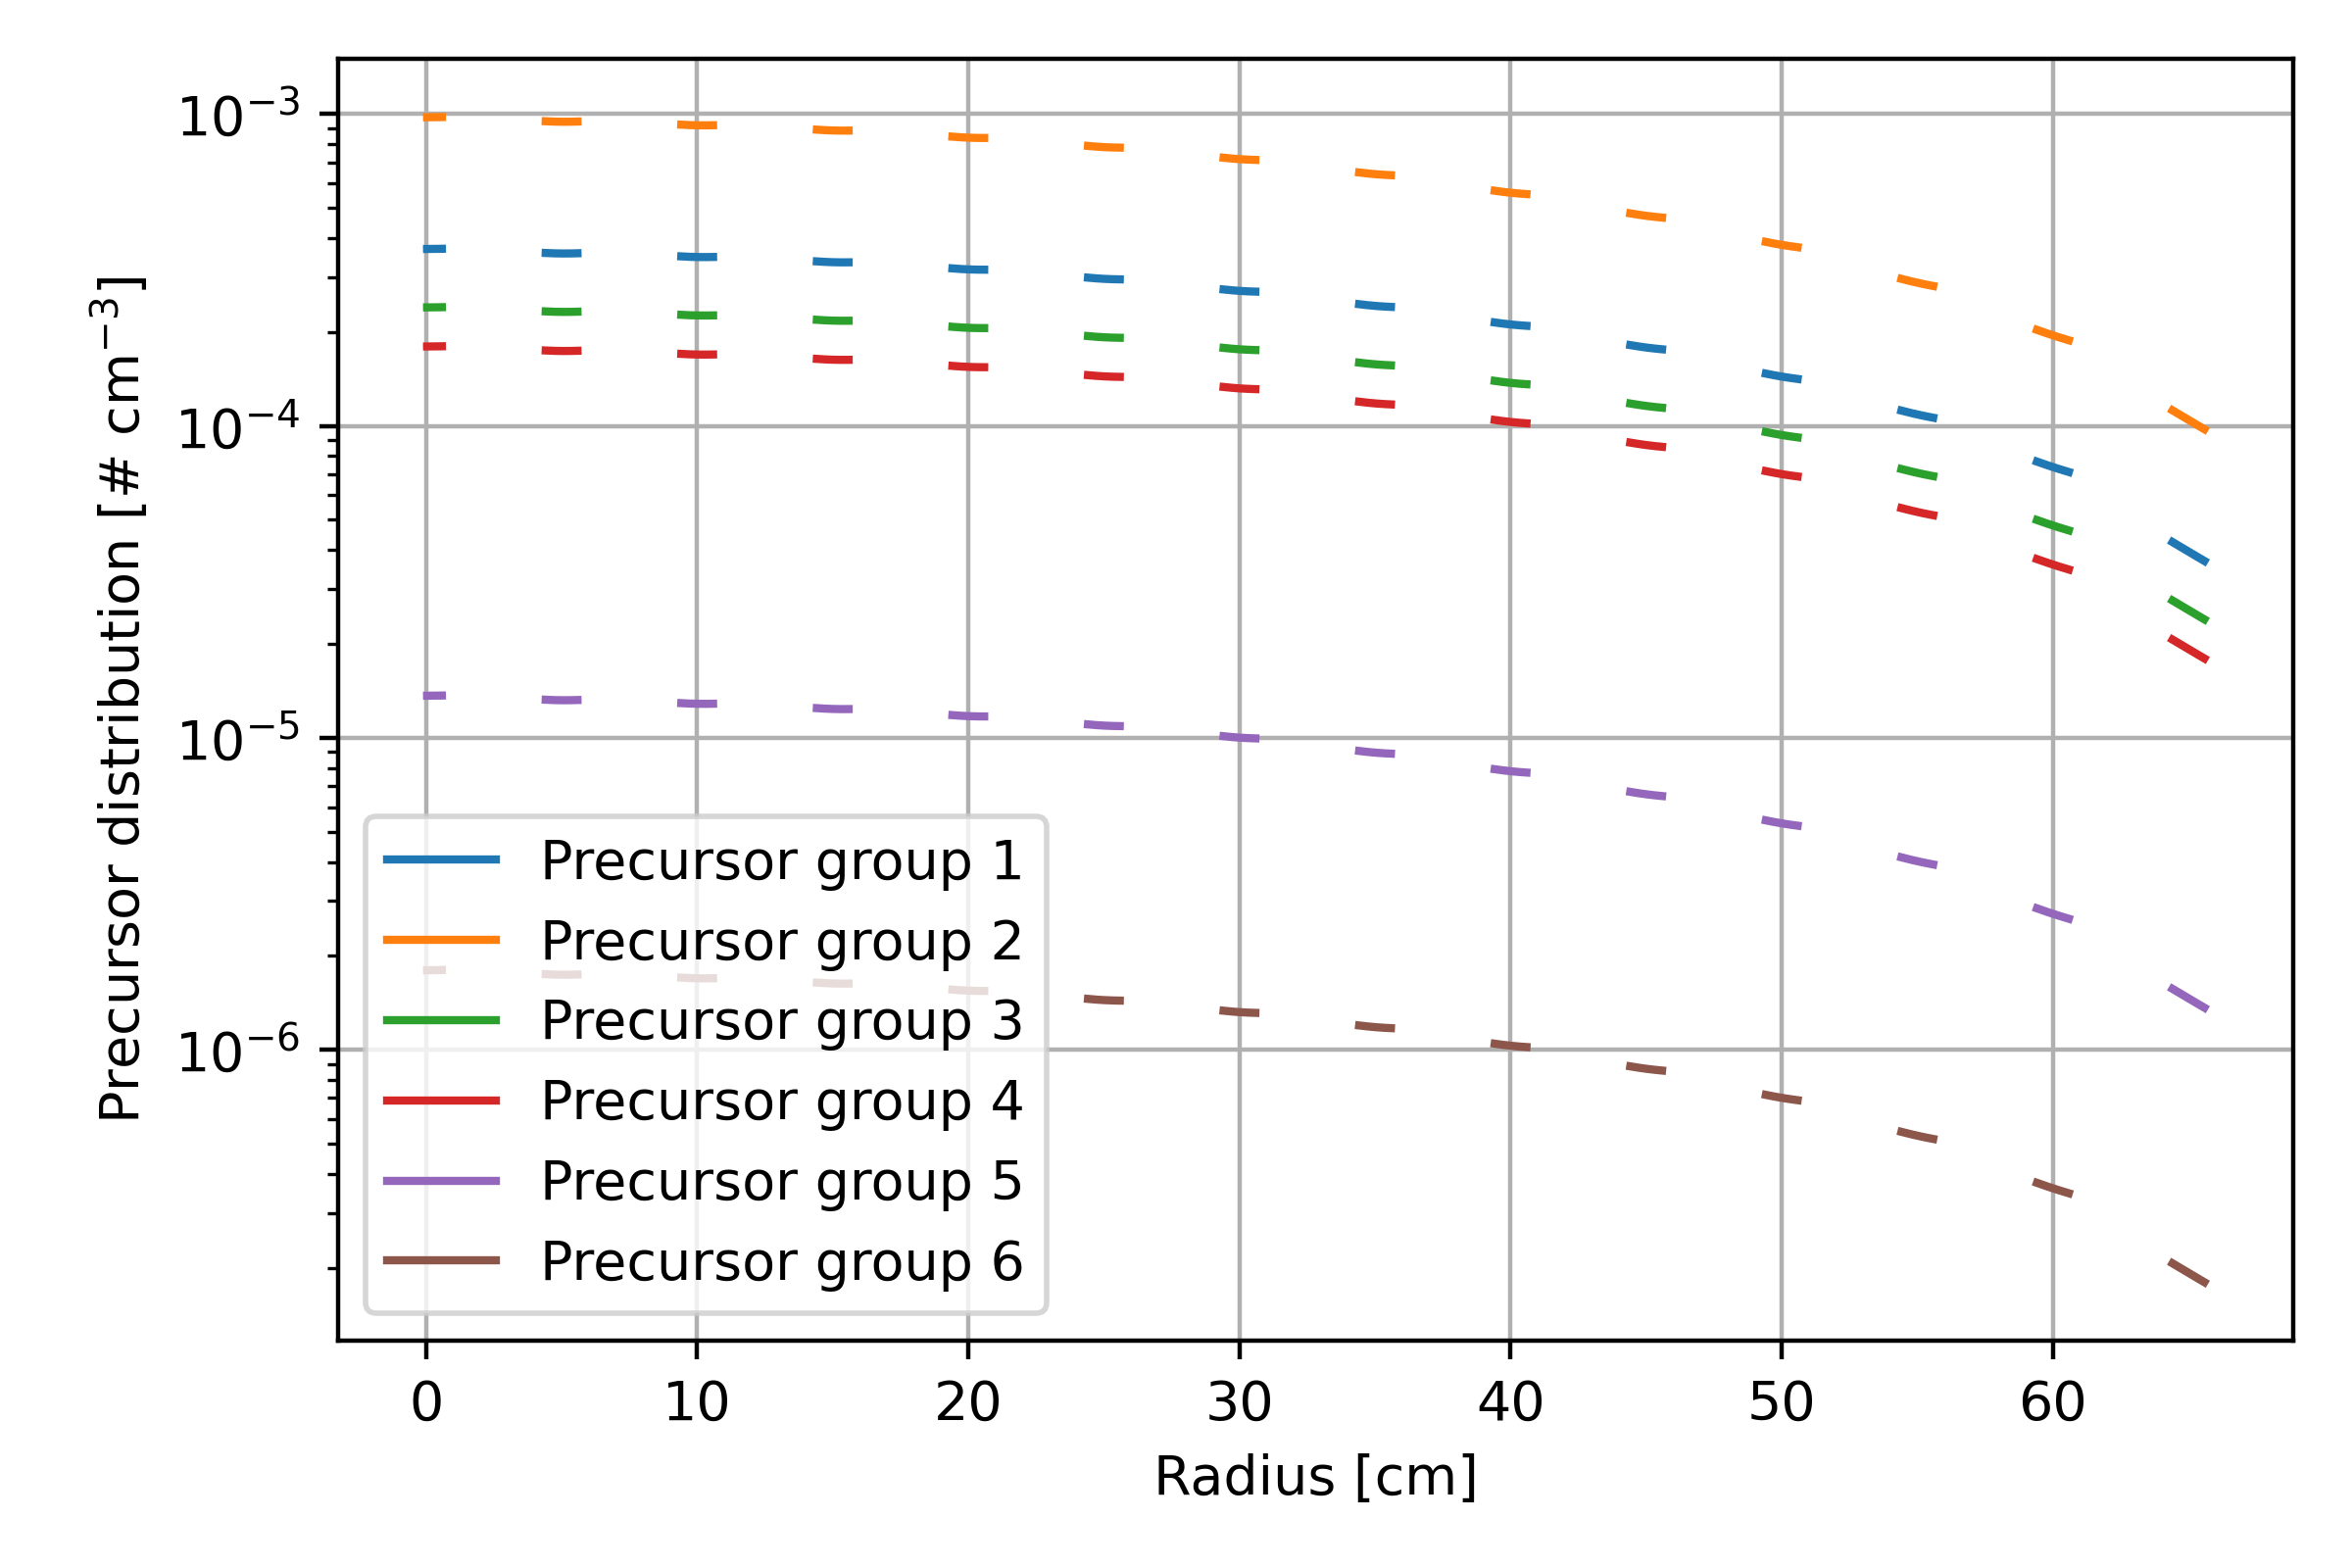
\includegraphics[width=\columnwidth]{midplane_pre}
    \caption{Normalized midplane \gls{DNP} distributions.}
    \label{fig:midplane-pre-dist}
  \end{subfigure}
  \hfill
  \begin{subfigure}[b]{0.48\columnwidth}
    \centering
    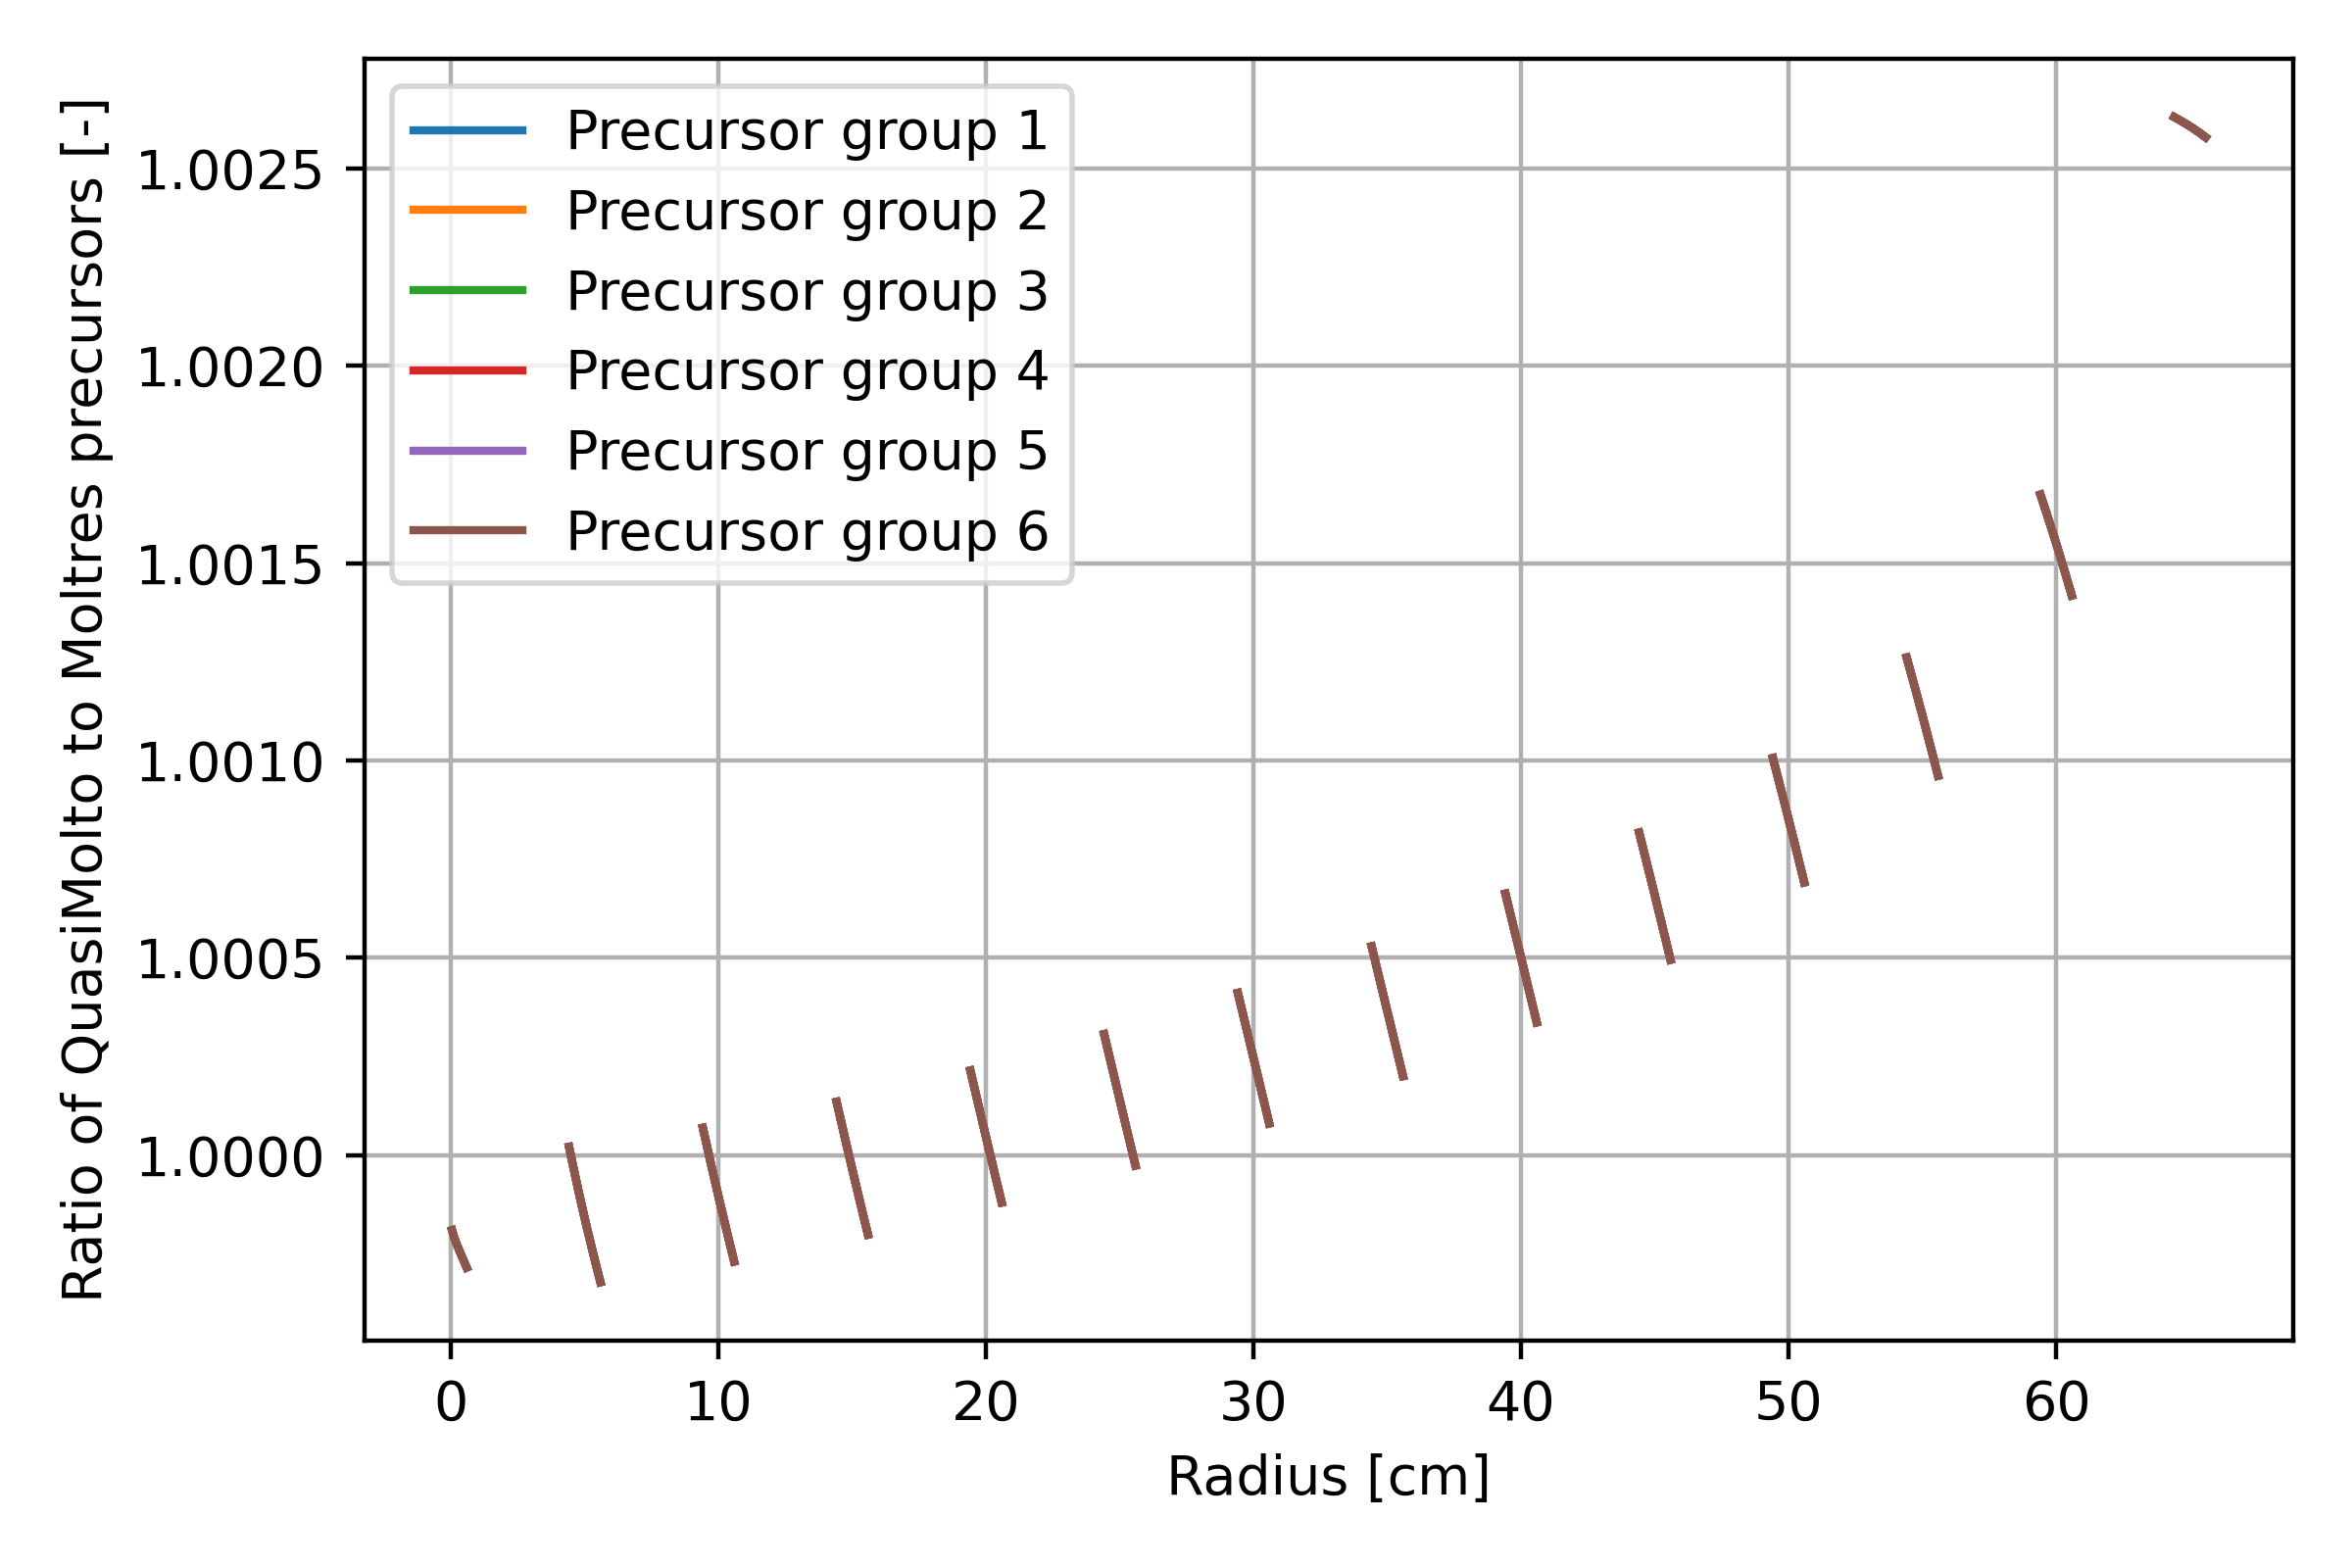
\includegraphics[width=\columnwidth]{midplane_pre_ratio}
    \caption{Ratio of midplane \gls{DNP} distributions.}
    \label{fig:midplane-pre-ratio}
  \end{subfigure}
  \caption{Midplane \gls{DNP} distribution from Moltres and ratios comparing QuasiMolto and Moltres
  models under static \gls{MSRE} conditions. \glspl{DNP} exist only in the fuel channel regions.
  The ratio curves overlap perfectly.}
  \label{fig:midplane-pre}
\end{figure}

\begin{figure}[t]
  \centering
  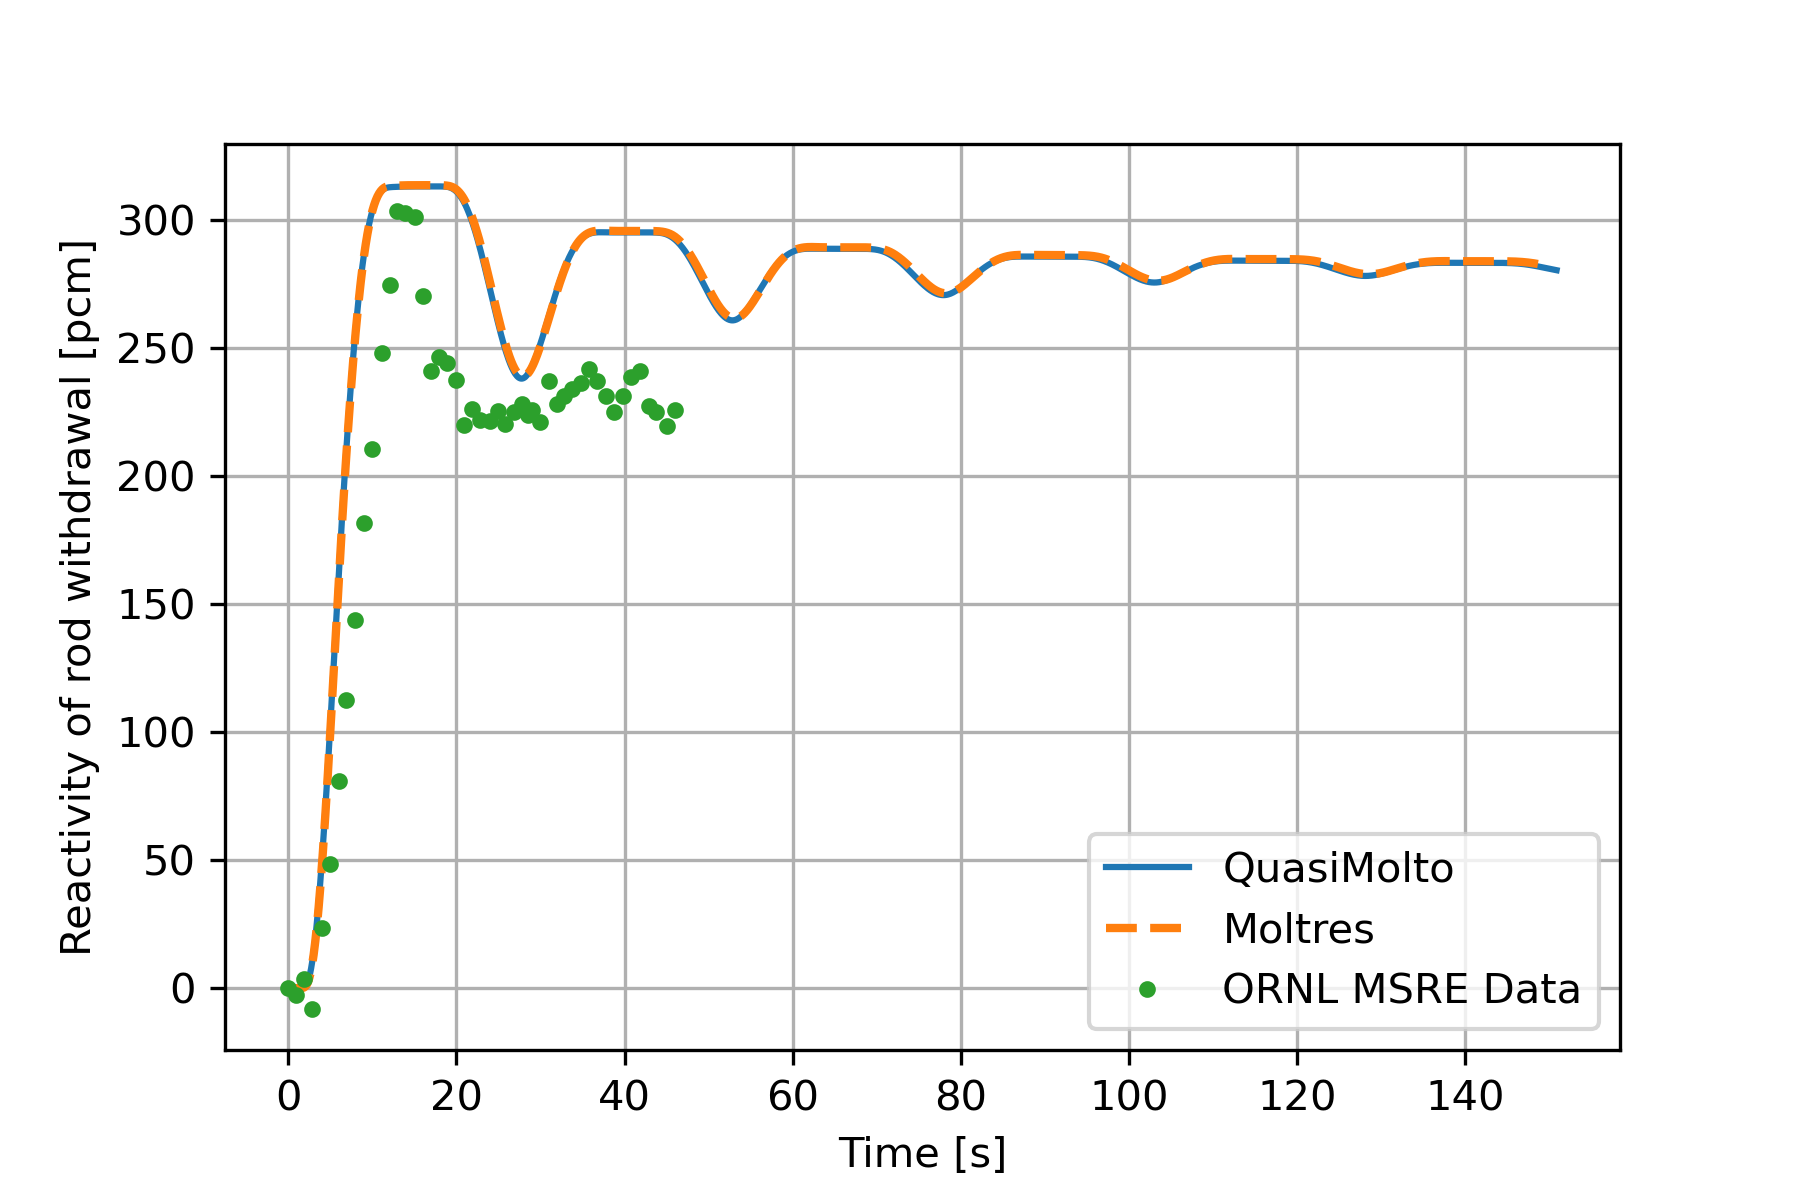
\includegraphics[width=0.8\columnwidth]{start-up-v2-reactivity}
  \caption{Reactivity loss (relative to static no-flow conditions) during the \gls{MSRE} pump
  start-up transient. The Moltres and QuasiMolto models agree closely with each other. The
  numerical models report greater peak and final reactivity change than the \gls{ORNL} \gls{MSRE}
  experimental data.}
  \label{fig:start-up-reactivity}
\end{figure}

Figure \ref{fig:start-up-reactivity} shows the change in reactivity loss relative to the static
condition during the pump start-up transient. Moltres and QuasiMolto report nearly identical
responses throughout the transient. Both codes and the \gls{ORNL} experimental data indicate a
steep increase in reactivity loss caused by the loss of \glspl{DNP} flowing out of the core with no
\glspl{DNP} flowing in. The reactivity loss peaks and plateaus starting around $t=12$ s for Moltres
and QuasiMolto and $t=13$ s for the \gls{ORNL} data. From the \gls{ORNL} data, the reactivity loss
drops after 2 s and stabilizes at around 225 pcm. From $t=30$ s onwards, the \gls{ORNL} reactivity
readings appear to be noisy with no obvious trend. In contrast, Moltres and
QuasiMolto report reactivity oscillations caused by the initial pocket of \gls{DNP} reentering the
core every salt recirculation cycle of 25.2 s. The oscillations eventually dissipate as the
\glspl{DNP} in the pocket progressively decay away over time. Reactivity loss from both codes
level out at around 282 pcm which is consistent with the reactivity change due to \gls{DNP} flow
from the steady salt flow case in Table \ref{table:msre-pump-keff}.

Three key differences stand out between the numerical results and \gls{ORNL} data. 1) The
\gls{ORNL} data logged a smaller reactivity loss of 225 pcm compared to 282 pcm from the
numerical results. 2) The \gls{ORNL} data logged a shorter reactivity loss plateau on the first
peak than the numerical results. 3) The \gls{ORNL} data did not log significant reactivity loss
oscillations after the first peak. These differences in the reactivity loss profile stem mainly
from the absence of upper and lower plena in the numerical model geometry (Figure
\ref{fig:pump-geom}).

Since the upper and lower plena comprise largely of salt, they retain some of the \glspl{DNP} which
we neglected in our numerical model geometry. Robertson \cite{robertson_msre_1965} reports that
salt residence times in the plena are approximately 4 s each. Therefore, Moltres and QuasiMolto
reported greater reactivity loss under steady flow conditions. With a combined salt residence time
of 17.1 s in the lower plenum, active core, and upper
plenum regions out of a full recirculation time of 25.2 s \cite{robertson_msre_1965}, there should
not be reactivity plateaus during the pump start-up transient. Lastly, Moltres and QuasiMolto
applied uniform salt flow and neglected turbulent mixing of \gls{DNP} in the plena and out-of-core
components. Without mixing, the numerical models preserved the initially static pocket of
\glspl{DNP} as it advected around the salt loop and produced the reactivity oscillations observed
in Figure \ref{fig:start-up-reactivity}. Conversely, the plateaus serve as
useful reference features for verifying advection modeling accuracy for code-to-code verification
in the context of \gls{MSR} simulations. This pump transient setup can be used to identify
advection schemes that suffer from excessive numerical diffusion or dispersion effects. The fact
that Moltres and QuasiMolto produced nearly identical results, despite significant differences in
their numerical schemes, lends credibility to both sets of results for the purpose of code
verification.

\begin{figure}[b]
  \centering
  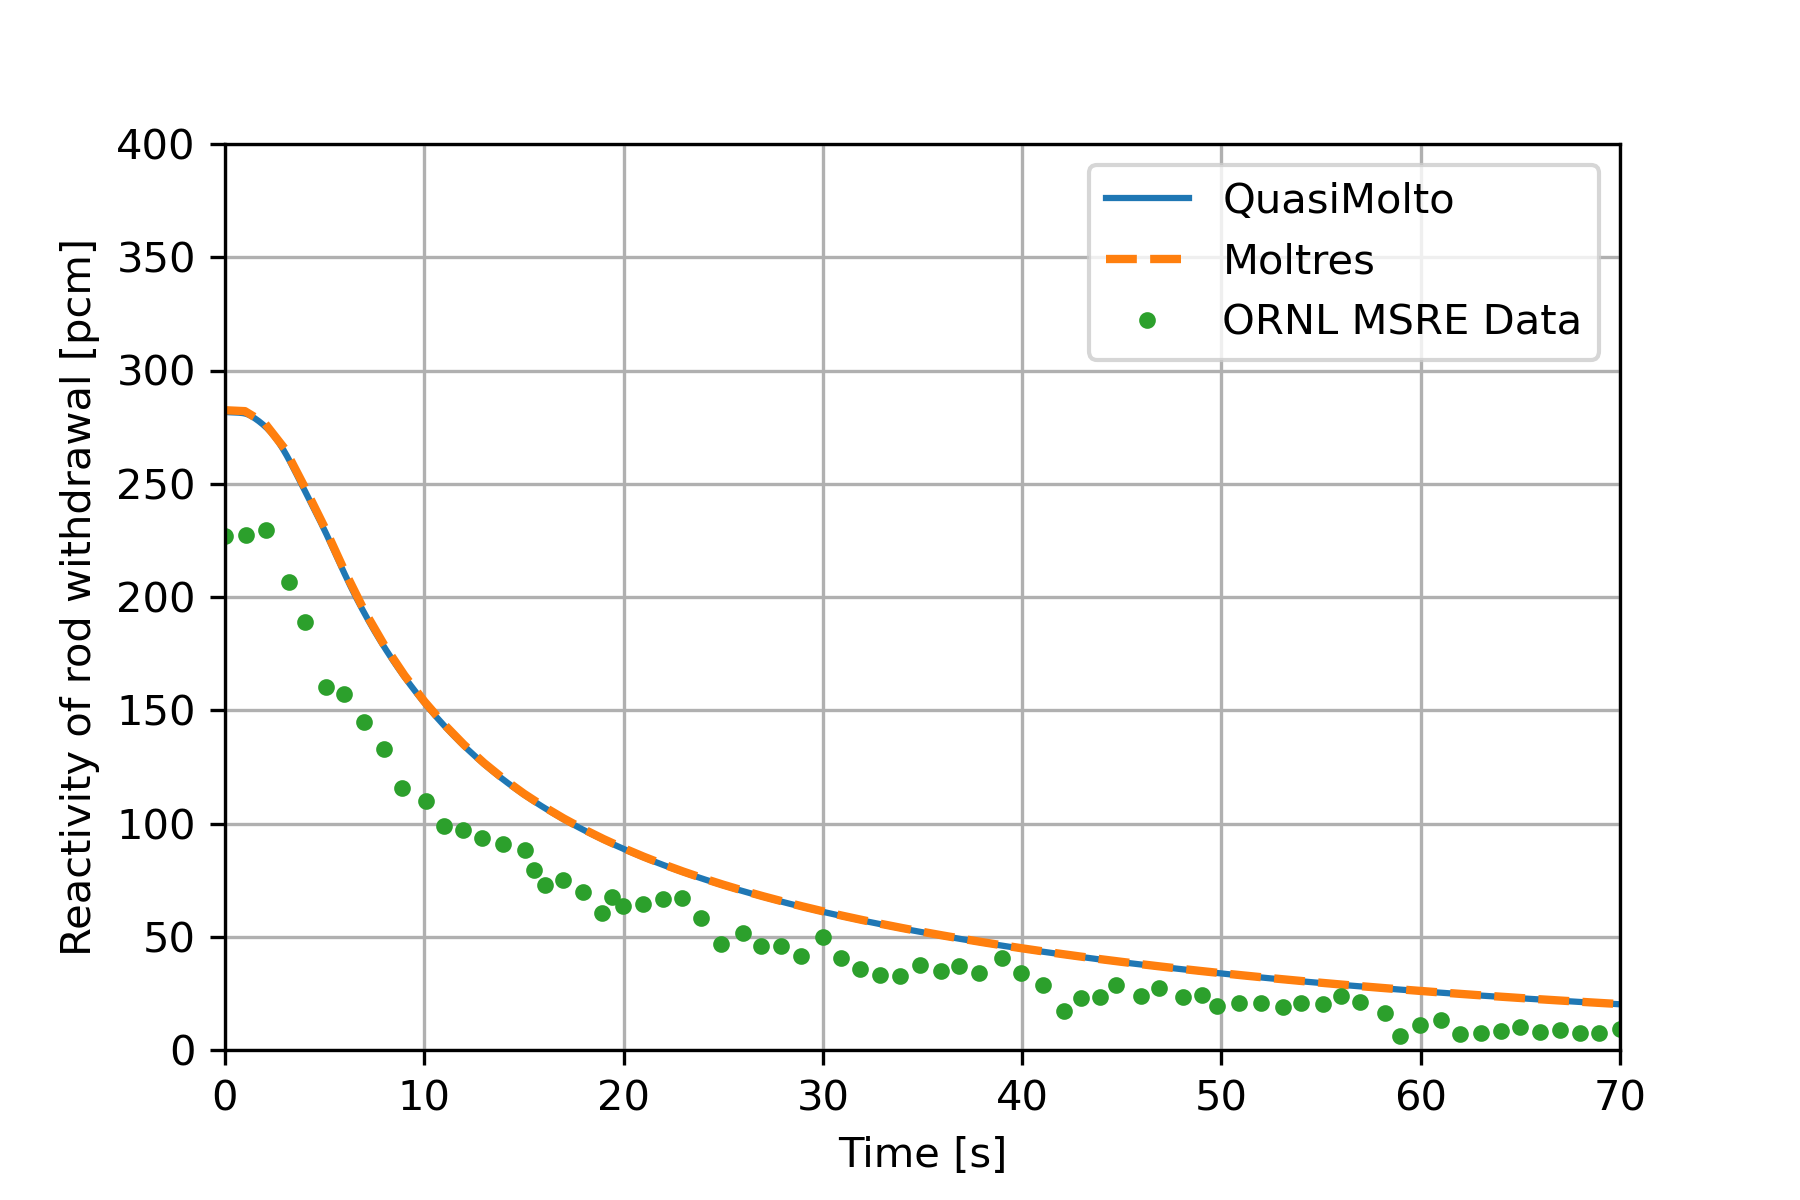
\includegraphics[width=0.8\columnwidth]{coast-down-v2-reactivity}
  \caption{Reactivity loss (relative to static no-flow conditions) during the \gls{MSRE} pump
  coast-down transient. The Moltres and QuasiMolto models agree closely with each other. The
  numerical models report greater reactivity change than the \gls{ORNL} \gls{MSRE} experimental
  data throughout the transient.}
  \label{fig:coast-down-reactivity}
\end{figure}

Compared to the pump start-up transient, the reactivity loss over time for the pump coast-down
transient shows a simpler, monotonic decline as shown in Figure \ref{fig:coast-down-reactivity}.
At the start of the transient, reactivity loss remains stable for 2 s due to inertia in salt flow.
Following this, the reactivity loss profile transitions into a steep exponential decline as
\glspl{DNP} accumulate in the increasingly stagnant salt. Other than the mismatch in reactivity
loss magnitude, Moltres and QuasiMolto reproduce the expected behavior observed in the \gls{ORNL}
pump coast-down data.

\subsection{Summary}

In collaboration with the developer of QuasiMolto \cite{reynolds_analysis_2023}, we performed a
\gls{VV} study based on the \gls{MSRE}
zero-power pump start-up and coast-down transient. This study was designed to assess
the looped \gls{DNP} flow modeling capabilities in Moltres and QuasiMolto reactor simulation
software. We used a 2-D axisymmetric model of the \gls{MSRE} to numerically model the pump
transients.

Moltres and QuasiMolto were consistent with each other in $k$-eigenvalue neutronics simulations
under static and steady salt flow conditions prior to pump transient simulations. The
$k_\text{eff}$ estimates from both codes were within 22 and 21 pcm of each other under the static
and steady flow conditions and the calculated reactivity loss due to \gls{DNP} flow agreed within
less than 1 pcm. The centerline and midplane flux and \gls{DNP} distributions showed nearly perfect
overlap with relative differences falling under 0.8\%.

Moltres and QuasiMolto remained consistent with each other in the pump start-up and
coast-down scenarios. Both codes reproduced most of the trends in reactivity loss from \gls{DNP}
flow observed in the \gls{ORNL}
\gls{MSRE} experimental data. Several differences between the numerical and experimental data arose
primarily due to the absence of upper and lower plena in the numerical model and the omission of
turbulent mixing. Nevertheless, the numerical results for the pump start-up transient
simulation captured distinct reactivity oscillations corresponding to the \gls{MSRE} salt
recirculation period. These oscillations served as valuable reference points for verifying \gls{DNP}
advection modeling accuracy between Moltres and QuasiMolto. Researchers looking to verify
their \gls{MSR} simulation software may use the results of this study as a benchmark.

\FloatBarrier
